\chapter{The systemic functional theory of grammar} %The systemic functional grammar}
\label{ch:sfg}

Any description of language requires a theory that provides the frame, scope and the necessary concepts. 
%used to describe a grammar i.e. structure, categories, functions, relations and how they relate to one another. 
Having a solid theory of grammar contributes to explaining what language is and how it works. It also frames how language is ought yo be analysed by either human or machines. 
%A grammar, as a description of linguistic rules, is thus framed by a theory of grammar expressing what language is, how it functions and in which ways it shall be describes.

In his seminal paper \citet{Halliday61} addresses the ardent need of the time for a general theory of language and partially answers the proposal for a universal theory of language. He sets out what was known at the time as Scale and Category Grammar. 
In such a model \textit{units} are set up to account for for pieces of language which carry grammatical patterns. They are seen as arranged on a hierarchical \textit{rank} scale of words, groups and clauses. These and other foundational concepts are covered in the first part of this Chapter. 

There are two variants of Systemic Functional Grammars: the \textit{Sydney Grammar} started in 1961 by \citet{Halliday2002} and the \textit{Cardiff Grammar} proposed by \citet{Fawcett2008} which is a simplification and an extension of the Sydney Grammar. To understand the underlying common motives and how they are different we shall start looking at their theories of grammar. They also have quite different historical developments. 

%Sydney theory of grammar originates with \citet{Halliday61-orig} defining the categories of the theory of grammar. It has been then  further refined in \citep{Halliday2003-systemic-theory} and in highly influential ``Introduction to Functional Grammar'' \citep{ifg}. Sydney grammar developed by \citet{Matthiessen-lexcartog-book} had been computationally implemented as part of a large scale natural language generation project called PENMAN \citep{PenmanOverview,Penman89}. It is worth noting that one of the well known SFG implementations for English, Nigel grammar \citep{intronigel}, was part of the same project.  
%Cardiff theory of grammar crystallised in ``A theory of syntax for Systemic Functional Linguistics'' \citep{Fawcett2000} which represents a large body of research part of the COMMUNAL project \citep{Fawcett90-communal,Fawcett93-ewnlg4} performed at Cardiff University.

Sydney and Cardiff grammars have been formalised to the point where they could be computationally applied to natural language generation. They have been implemented in PENMAN \citep{PenmanOverview,Penman89} and respectively COMMUNAL projects \citep{Fawcett90-communal}. Both versions of SF grammars have been used predominantly for English and implementations of for other languages are also available. The major component of PENMAN is a computer model of Halliday's SF grammar described by \citet{gazebo}, \citet{MatthiessenBateman91}, \citep{Matthiessen-lexcartog-book} and others. COMMUNAL is the computer implementation of Cardiff grammar described by \citet{Fawcett:1988}, \citet{Fawcett93-ewnlg4} and others. 

This chapter first sets out the basic organisational dimensions for each of the theories and then discusses comparatively Halliday's \citep{Halliday2002} and Fawcett's \citep{Fawcett2000} versions of SFL.

%Because SFL grammar works with more complex structures than simply word dependencies like Dependency Grammars therefore the pragmatics of this chapter is at large oriented towards describing what constituents and functions can be derived from dependency structure and word classes and what is beyond that of a more semantic nature.

\section{A word on wording}
\label{sec:wording}
Before going into deeper discussion I first make terminological clarifications on the terms: grammar, grammatics, syntax, semantics and lexicogrammar. I start with a definitions adopted in ``mainstream'' generative linguistics and then present how the same terms are discussed in systemic functional linguistics.

%Radford1997: A minimalist introiduction to syntax
Radford, a generative linguist, in the ``Minimalist Introduction to Syntax'' (\citeyear{Radford1997}), starts with a description of grammar as a field of study, which, in his words, is traditionally subdivided into two inter-related areas of study: syntax and morphology. %\citep[1]{Radford1997}.

\begin{definition}[Morphology (Radford)]\label{def:morphology-min}
Morphology is the study of how words are formed out of smaller units (traditionally called morphemes) \citep[1]{Radford1997}.
\end{definition}

\begin{definition}[Syntax (Radford)]\label{def:syntax-min}
Syntax is the study of how words can be combined together to form phrases and sentences. \citep[1]{Radford1997}
\end{definition}

%In London school of linguistics this distinction is perceived as unnecessary. %Halliday (on grammar) 2002 
%He take this position to motivate the proposed SFG architecture.
Halliday, in the context of \textit{rank} scale discussion (see Definition \ref{def:constituency-principles} and \ref{def:rank-skale-constraints}), refers to the traditional meaning of syntax as the \textit{grammar above the word} and to morphology as \textit{grammar below the word} \citep[ 51]{Halliday2002}. Such a distinction, he states, has no theoretical status and is deemed as unnecessary distinction. Halliday adopts this position to motivate the architecture of grammar he was developing and is inherited from his precursor, Firth, as he puts it: 
\begin{quote}
	\dots the distinction between morphology and syntax is no longer useful or convenient in descriptive linguistics. \citep[14]{Firth1957}
\end{quote}

%[JB] if you say that this is Halliday's position and was used to motivate the architecture of SFG, then no one can complain or disagree, because that is simply a statement of fact.
%[JB] Morphology works with very different principles to syntax (that is why in our versions of many grammar, we have such different realisation rules for morphology and for syntax). 

Radford adds that, traditionally, grammar is not only concerned with the principles governing formation of words, phrases and sentences but also with principles governing their interpretation. Therefore \textit{structural aspects of meaning} are said to be also a part of grammar. 

\begin{definition}[Grammar (Radford)]\label{def:grammar-min}
[Grammar is] the study of the principles which govern the formation and interpretation of words, phrases and sentences. \citep[1]{Radford1997}
\end{definition}

Interestingly enough, the Definition \ref{def:grammar-min} makes no mention at all to the lexicon. This is because the formal grammars focus primarily on unit classes and how they are accommodated in various structures and so in formal linguistics the lexicon is often disconnected from the grammar. The systemic grammar, on the other hand, along with formal descriptions of grammatical categories and structures, includes the lexicon as part of grammar to form a \textit{lexicogrammar}. At this point I have to mention that systemic functional grammar is not the only lexicalised one and there are others taking the same approach such as 
%TODO: references needed
Lexical Functional Grammar (LFG), Head Phrase Structure Grammar (HPSG), Combinatory Categorial Grammar (CCG) and others. 

Another important aspect to notice is that the grammar is defined as a field of study rather than a set of rules. De divergence in perspective on the subject led Halliday, since his early papers, to become conscious the difference between a study of a phenomenon with the phenomenon itself. By analogy to language as phenomenon and linguistics as the study of the phenomenon, discussed in  \citep{Halliday1997-linguistics}, Halliday adopts the same wording for \textit{grammar} as phenomenon and \textit{grammatics} as the study of grammar; the same distinction holds for \textit{syntax} and \textit{syntactics}.

\begin{definition}[Grammatics (Halliday)]\label{def:grammatics-halliday}
	Grammatics is a theory for explaining grammar \citep[369]{Halliday2002}
\end{definition}

%E. Moravcsik
Moravcsik, another generative linguist, stresses the same distinction, in her ``An introduction to syntax'' \citep{Moravcsik2006}, and presents two ways in which the word \textit{syntax} is used in the literature: (a) in reference to a particular aspect of grammatical structure and (b) in reference to a sub-field of descriptive linguistics that describes this aspect of grammar. 
In her words: 

\begin{quote}
	\dots
	syntax describes the selection and order of words that make well-formed sentences and it does so in as general a manner as possible so as to bring out similarities among different sentences of the same language and different languages and render them explainable. \dots syntax rules also need to account for the relationship between string of word meanings and the entire sentence meaning, on one hand, and relationship between strings of word forms and the entire sentential phonetic form, on the other hand. \citep[25]{Moravcsik2006}	
\end{quote}

In her definition of grammar she includes the lexicon and semantics which is a somewhat more explicit statement than Radford's \textit{interpretation}. She is also getting, in Definition \ref{def:grammar-moravcsik}, somewhat closer to what grammar stands for in SFL - Definition \ref{def:grammar-halliday}. 

\begin{definition}[Grammar (Moravcsik)]\label{def:grammar-moravcsik}
... maximally general analytic descriptions, provided by descriptive linguistics, [are] called grammars. A grammar has five components: phonology (or, depending on the medium, its correspondent e.g. morphology), lexicon, syntax and semantics\citep[24--25]{Moravcsik2006}. 
\end{definition}

%Halliday and Matthiessen 1999 - Construing experience through meaning

%Halliday (on grammar) 2002
\begin{definition}[Grammar (Halliday)]\label{def:grammar-halliday}
	To Halliday, lexico-grammar, or for short,simply grammar is a part of language and it means the wording system - the ``lexical-grammatical stratum of natural language as traditionally understood, comprising its syntax, vocabulary together with any morphology the language may display [...]'' \citep[369]{Halliday2002}.
\end{definition}

%Another important aspect to note about the generative linguistics is the focus on the formal aspects of language where even the semantics (also referred to as interpretation) refers only to the ``formal aspect of meaning''. 

The last point I want to mention is the approach to semantics. Formal grammars aim to account for the realisation variations, that is formation of words, phrases and sentences along with their arrangements and mention of semantics is often restricted to what may be termed the \textit{formal aspect of meaning}. 

By contrast, a systemic grammar is a functional grammar, which means (among other things) that it is semantically motivated, i.e. ``natural''. 
%TODO: [JB] note that most contemporary theories of grammar assume a close morphism betwene grammar and semantics - this is then also 'natural' (even more generally, this is the long acknowledged operation of iconicity in grammar), so be careful what you state as being about grammar and what is meant to be specific about 'SFG'.
So the fundamental distinctions between formal and functional grammars is the semantic basis for explanations of structure. 
%TODO: [JB] Here you might be better going back to Butler's definitions and distinctions btween formal and functional grammars, as the boundary is by no means clearcut. The way you have it, most modern formal linguists would be alienated: think of CCG, there the relation between semantics and grammar is enforced even more strongly than in SFG: each and every grammar rule is at the same time a semantic rule. This is also in Montague grammar and so is not new. I would phrase these things by placing the basic assumptions of SFG as running alongside these assumptions, not as a distinction that separates SFG from them.

Also, in SFL, the meaning is being approached from a semiotic perspective, placing the linguistic semantics in perspective with the linguistic expression and the real world situation. 
In this respect, \citet{Lemke93} offers a well formulated theoretical foundation that ``human communities are eco-social systems that persist in time through ongoing exchange with their environment; and the same holds true for any of their sub-subsystems [...]'' including language. The social practices constituting such systems are both material and semiotic, with a constant dynamic interplay between the two. \citep[387]{Halliday2002}

To Halliday, the term \textit{semiotic} accounts for an orientation towards meaning rather than sign. In other words, the interaction is between \textit{the practice of doing and the practice of meaning}. As the two sets of practices are strongly coupled, Lemke points out that there is a high degree of redundancy between the \textit{material-semiotic interplay}. And it perfectly resonates with Firth's idea of \textit{mutual expectancy} between the text and the situation. This idea of interplay is incorporated in SFL as \textit{language stratification} and is graphically represented in Figure \ref{fig:stratification-sfl}.

\begin{figure}[h]
	\centering
	\begin{tikzpicture}
		\coordinate (o) at (0,0);
		\coordinate (o-11) at (-16em,16em);
		
		\coordinate (A) at (-9,2);
		\coordinate (C) at (-6,6);
		\coordinate (D) at (-1,1);
		
		\draw[thick, name path = mn] (o) arc(315:-360:4em);
		\draw[thick, name path = me](o) arc(315:-360:7em);
		\draw[thick, name path = mx] (o) arc(315:-360:10em);
		
		\draw[thin, white, name path = ref](o)--(o-11);
		
		\path[name intersections={of = ref and mn, name = tgt} ];
		\draw[thick, dashed, name path = plane] ($(tgt-2)!10em!90:(C)$) -- ($(tgt-2)!14em!-90:(C)$);
		\path[name intersections={of = plane and mx, name = tgt2} ];
		
		\draw[thick, <->, postaction={ decorate ,decoration = {text along path, raise=1ex, text align=center,text={Stratification}}}](A) -- +($(D)-(C)$);  % the stratification axis line
		
		\node[align = center] at (-1,1) {Phonology \\ (sounding)};
		\node[align = center] at (-3,3) {Lexicogrammar \\ (wording)};
		\node[align = center] at (-5,5) {Semantics \\ (meaning)};
		
		\node[align = center] at (2,5) {Expression};
		\node[align = center] at (0.4,6.6) {Content};
		
		\coordinate (ec) at (-0.6,2) ;
		
%		\draw[red, fill = red](tgt-1) circle(0.1em);
%		\draw[red, fill = red](tgt-2) circle(0.1em);
%		\draw[red, fill = red](tgt2-1) circle(0.1em);
%		\draw[red, fill = red](tgt2-2) circle(0.1em);
		
		%\fill[yellow, fill opacity=.4] (o) arc(315:393.5:10em) -- (tgt-2) arc (135:300:4em);
		\fill[yellow, fill opacity=.2] (o) arc(315:393.5:10em) -- (tgt2-1) arc (236.5:315:10em);
		
	\end{tikzpicture}
	\caption{The levels of abstraction along the realisation axis}
	\label{fig:stratification-sfl}
\end{figure}
 

Having that said, the stratification axis is a useful dimension to relate the formal and the systemic functional grammars. This is also an instrument employed by Hjelmslev \citep{Taverniers2011}. %TODO: eventually expand here

The SFL model defines language as a resource organised into three strata: phonology (sounding), lexicogrammar (wording) and semantics (meaning). Each is defined according to its level of abstraction on the realisation axis. The realisation axis is divided into two planes: the expression and the content planes. 
Although debate about the precise division continues, for current purpose it is sufficient to see the first stratum (i.e. phonology/morphology) belongs to the \textit{expression plane} and the last two (lexicogrammar and semantics) belong to the \textit{content plane}.
%But the division is not so clear because some parts of semantics and lexicogrammar transcend from content into expression plane. 
In this context, the formal grammar could be localised entirely within the expression plane, including the phonology/morphology, syntax, lexicon while formal semantics, stripped of any explanations in terms of the meaning potential, belongs in the content plane.

\section{Sydney theory of grammar}
\label{sec:sydney-theory-of-grammar}
I start introducing the terms of SFL theory with the Sydney grammar as this is in accordance with the historical development originating with \citet{Halliday2002} defining the categories of the theory fo grammar. He proposes four fundamental categories: \textit{unit}, \textit{structure}, \textit{class} and \textit{system}. Each of these categories is logically derivable from and related to the other ones in a way that they mutually define each other. These categories relate to each other on three scales of abstraction: \textit{rank}, \textit{exponence}, \textit{delicacy}. Halliday also uses three scale types: \textit{hierarchy}, \textit{taxonomy} and \textit{cline}.

\begin{definition}[Hierarchy]\label{def:hierarchy}
	Hierarchy [is] a system of terms related along a single dimension which involves some sort of logical precedence. 
	\citep[42]{Halliday2002}. 
\end{definition}

\begin{definition}[Taxonomy]\label{def:taxonomy}
	Taxonomy [is] a type of hierarchy with two characteristics:
	\begin{enumerate}
		\item the relation between terms and the immediately following and preceding one is constant
		\item the degree is significant and is defined by the place in the order of a term relative to following and preceding terms. \citep[42]{Halliday2002}
	\end{enumerate}
\end{definition} 

\begin{definition}[Cline]\label{def:cline}
	Cline [is] a hierarchy that instead of being made of a number of discrete terms, is a continuum carrying potentially infinite gradations.
	\citep[42]{Halliday2002}. 
\end{definition}

The concept of cline may not necessarily originate in SFL but it is used quite extensively in the domain literature.
Next I define and introduce each category of \textit{grammatics} and the related concepts that constitute the theoretical foundation for the Sydney Theory of grammar.
%TODO [JB] note how you've already lost the other three terms you had above: rank, exponence and delicacy. Either define them immediately or say where they are going to be defined.

\subsection{Unit}
\label{sec:unit-sydney}
Language is a patterned activity of meaningful organization. The patterned organization of substance (\textit{graphic} or \textit{phonic}) along a linear progression is called \textit{syntagmatic order} (or simply \textit{order}). 

\begin{definition}[Unit]\label{def:unit}
	The unit is a grammatical category that accounts for the stretches that carry grammatical patterns \citep[42]{Halliday2002}.
	The units carry a fundamental \textit{class} distinction and should be fully identifiable in description \citep[45]{Halliday2002}.
\end{definition}

\begin{generalization}[Constituency principles]\label{def:constituency-principles}
	The five principles of constituency in lexicogrammar are:
	\begin{enumerate}
		\item There is a scale or rank in the grammar of every language. That of English (typical of many) can be represented as: clause, group/phrase, word, morpheme.
		\item Each unit consists of \textit{one or more} units of rank next below.
		\item Units of every rank may form complexes.
		\item\label{item:downrank} There is potential for rank shift, whereby a unit of one rank my be down-ranked to function in a structure of a unit of its own rank or of a rank below.
		\item\label{item:unit-split} Under certain circumstances it is possible for one unit to be enclosed within another, not as a constituent but simply in such a way as to split the other into two discrete parts \citep[9--10]{Halliday2013}.
	\end{enumerate}
\end{generalization}

For example, the down-ranking (Point \ref{item:downrank}) can be observed in nominal groups that incorporate a relative clause functioning as qualifier. In example \ref{ex:downranking} \textit{that I got for Christmas} is a relative clause specifying which books are being referred. The unit split (Point \ref{item:unit-split}) can be encountered in the instances of Wh-interrogative clauses containing a preposition at the end which in fact belongs to the Wh-group. In example \ref{ex:unit-split2} the prepositional phrase \textit{Who \dots about} is gapped and has an inverted order of constituents. 

%TODO: write 2 examples here

\begin{exe}
	\ex\label{ex:downranking} I haven't read any books \textit{that I got for Christmas}.
	\ex\label{ex:unit-split2} \textit{Who} are you talking \textit{about}?
	\ex\label{ex:unit-split1} I am talking about George.
\end{exe}

The relation between units is that of consistency for which we say that a unit \textit{consists of} other units. The scale on which the units are ranged is the \textit{rank scale}. The rank scale is a levelling system of units supporting unit composition regulating how units are organised at different granularity levels from clause, to groups/phrases to words and the units of a higher rank scale consist of units of the rank next below. Table \ref{tab:rank-scale} presents a schematic representation of the rank scale and its derived complexes.

\begin{table}[h]
	\centering
	\begin{tabular}{|l|l|}
		\hline
		{\bf Rank scale $\downarrow$} & {\bf Complexing} \\ \hline
		& Clause complex           \\ \hline
		Clause           &                          \\ \hline
		& Group(/phrase) complex   \\ \hline
		Group(/phrase)   &                          \\ \hline
		& Word complex             \\ \hline
		Word             &                          \\ \hline
		& (Morpheme complex)       \\ \hline
		(Morpheme)       &                          \\ \hline
	\end{tabular}
	\caption{Rank scale of the (English) lexicogrammatical constituency}
	\label{tab:rank-scale}
\end{table}

\begin{generalization}[Rank scale constraints]\label{def:rank-skale-constraints}
	The rank relations are constrained as follows:
	\begin{enumerate}
        \item in general elements of clauses are filled by groups,the elements of groups by words and the elements of words by morphemes.
		\item downward \textit{rankshift} is allowed i.e. the transfer of a given unit to a lower rank. 
		\item upward rankshift is not allowed.
		\item only whole units can enter into higher units \citep[44]{Halliday2002}.
	\end{enumerate}
\end{generalization}

The Generalization \ref{def:rank-skale-constraints} taken as a whole means that a unit can include, in what it consists of, a unit of rank higher than or equal to itself but not a unit of rank more than one degree lower than itself; and not in any case a part of any unit \citep[42]{Halliday2002}. 

Following the rank scale constraints above the concept of embedding can be defined as follows. 

\begin{definition}[Embedding]\label{def:embedding0}
    Embedding is the mechanism whereby a clause or phrase comes to function as a constituent within the structure of a group, which is itself a constituent of a clause. \citep[242]{Halliday2013}
\end{definition}

Halliday states that embedding is a phenomena that occurs only when a phrase/group or clause function within the structure of a group which is itself a constituent of a clause \citep[242]{ifg2}. The above definition of embedding permits the only for a clause and groups that function as elements of groups which means that a clause cannot fill the elements of another clause \citep[237]{Fawcett2000}.

\subsection{Structure}
\label{sec:structure-sydney}
%TODO: Top down is good for generation and bottom up for parsing
%TODO: agnation as a clive vs instanciation as a cline | subclassification rel vs class-instance rel
%TODO: Rebekah Wegener PhD SFL thesis online [Parameters of context]: Chapter in SFL theory 

\begin{definition}[Structure]\label{def:structure}
	The structure (of a given unit) is the arrangement of \textit{elements} that take places distinguished by the order relationship \citep[46]{Halliday2002}.
\end{definition}

\begin{definition}[Element]\label{def:element}
	Element is defined by the place stated as absolute or relative position in sequence and with reference to the unit next below \citep[47]{Halliday2002}. 
\end{definition}


\begin{figure}[h]
	\begin{tikzpicture}
		\tikzset{
			rect/.style n args={4}{
				draw=none,
				rectangle,
				append after command={
					\pgfextra{%
						\pgfkeysgetvalue{/pgf/outer xsep}{\oxsep}
						\pgfkeysgetvalue{/pgf/outer ysep}{\oysep}
						\def\arg@one{#1}
						\def\arg@two{#2}
						\def\arg@three{#3}
						\def\arg@four{#4}
						\begin{pgfinterruptpath}
						\ifx\\#1\\\else
						\draw[draw,#1] ([xshift=-\oxsep,yshift=+\pgflinewidth]\tikzlastnode.south east) edge ([xshift=-\oxsep,yshift=0\ifx\arg@two\@empty-\pgflinewidth\fi]\tikzlastnode.north east);
						\fi\ifx\\#2\\\else
						\draw[draw,#2] ([xshift=-\pgflinewidth,yshift=-\oysep]\tikzlastnode.north east) edge ([xshift=0\ifx\arg@three\@empty+\pgflinewidth\fi,yshift=-\oysep]\tikzlastnode.north west);
						\fi\ifx\\#3\\\else
						\draw[draw,#3] ([xshift=\oxsep,yshift=0-\pgflinewidth]\tikzlastnode.north west) edge ([xshift=\oxsep,yshift=0\ifx\arg@four\@empty+\pgflinewidth\fi]\tikzlastnode.south west);
						\fi\ifx\\#4\\\else
						\draw[draw,#4] ([xshift=0+\pgflinewidth,yshift=\oysep]\tikzlastnode.south west) edge ([xshift=0\ifx\arg@one\@empty-\pgflinewidth\fi,yshift=\oysep]\tikzlastnode.south east);
						\fi
						\end{pgfinterruptpath}
					}
				}
			}, 
			unit/.style={rect={draw=black, thick}{draw=black, thick}{draw=black, thick}{}},
			place/.style = {rect={draw=black, thick}{}{draw=black, thick}{draw=black, thick}, text width=5.5em,},
			}
		
		\node[unit, text width=\textwidth,align=center](unit-line){};
		\node[above = 0.1em of unit-line](unit-label){Unit};
		%place lines
		{[start chain=l going left,node distance=1em]
			\node[on chain=l,place, below =3em of unit-line](p1){};
			\node[on chain=l,place](p2){};
			\node[on chain=l,place](p3){};
		}
		%place lines to the right
		{[start chain=r going right, node distance=1em,]
			\node[on chain=r,place, right = 1em of p1.east](p4){};
			\node[on chain=r,place](p5){};
			}
		%place labels
		\node[below=0.1em of p1](l3){place_{3}};
		\node[below=0.1em of p2](l2){place_{2}};
		\node[below=0.1em of p3](l1){place_{1}};
		\node[below=0.1em of p4](l4){place_{4}};
		\node[below=0.1em of p5](l5){place_{5}};
		%functional elements
		\node[above = 0.4em of p1, align=center, rectangle, draw, thick,dashed](element1){functional\\element_{3}};
		\node[above = 0.4em of p2, align=center, rectangle, draw, thick,dashed](element2){functional\\element_{2}};
		\node[above = 0.4em of p3, align=center, rectangle, draw, thick,dashed](element3){functional\\element_{1}};
		\node[above = 0.4em of p4, align=center, rectangle, draw, thick,dashed](element4){functional\\element_{4}};
		\node[above = 0.4em of p5, align=center, rectangle, draw, thick,dashed](element5){functional\\element_{5}};
		%order relations
		\draw[bend right,<->,dashed]  (l1) to node [below] {order} (l2);
		\draw[bend right,<->,dashed]  (l2) to node [below] {order} (l3);
		\draw[bend right,<->,dashed]  (l3) to node [below] {order} (l4);
		\draw[bend right,<->,dashed]  (l4) to node [below] {order} (l5);
	\end{tikzpicture}
	\caption{The graphic representation of (unit) structure}
	\label{fig:structure-representation}
\end{figure}

We say that a unit is composed of elements located in places and that its internal structure is accounted for elements in terms of functions and places taken by the lower (constituting) units or lexical items. The graphic representation of the unit structure is depicted in Figure \ref{fig:structure-representation}. The unit structure is referred in linguistic terminology as \textit{constituency} (whose principles are enumerated in Generalization \ref{def:constituency-principles}). In the unit structure, the elements resemble an array of empty slots that are \textit{filled} by other units or lexical items.

For example to account for the English clause structure four elements are needed: \textit{subject}, \textit{predicator}, \textit{complement} and \textit{adjunct}. They yield the distinct symbols, so that S, P, C, A is the inventory of elements. They then can be arranged in various orders falling in particular places, say SPC, SAPA, ASPCC etc. The places of elements are important with respect to the structure of the whole unit but also with respect to the relative ordering between these elements. For example S always fronts P, C is fronted by P unless the clause realises a Wh-interrogative whereas A is quite free and can occur anywhere in the unit structure. 

\subsection{Class}

To one place in the structure corresponds one occurrence of the unit next below. This means that there will be a certain grouping of members identified by the functional element they take in the structure. Patterning such groupings leads to emergence of \textit{classes} of units.

In the clause structure example, elements in the unit are occupied by units of lower rank and of a particular class. The relation between the element and the class is mutually determined. In each of these elements is placed a lower rank unit and of an expected class. For instance in the S position can be placed a \textit{noun}, \textit{nominal group}, \textit{pronoun} or another \textit{clause} (that will be a down-ranking situation defined above).

\begin{definition}[Class]\label{def:class}
	The class is that grouping of members of a given unit which is defined by the operation (i.e. functional element) in the structure of the unit next above \citep[49]{Halliday2002}.
\end{definition}

Halliday defines class (Definition \ref{def:class}) as likeness of the same rank \textit{phenomena} to occur together in the structure. He adopts a top-down approach stating that the class of a unit is determined by the \textit{function} (Definition \ref{def:function}) it plays in the unit above and not by its internal structure of elements. In SFG the structure of each class is well accounted in terms of syntactic variation recognizing six unit classes: \textit{clause}, \textit{nominal}, \textit{verbal}, \textit{adverbial} and \textit{conjunction} groups and \textit{prepositional phrase}. The Sydney unit structure model is briefly summarised in the Appendix \ref{ch:syntax-overview}.
%TODO: bring the Appendinx into the chapter structure

Halliday identifies the concept of \textit{grammatical metaphor} defined in \ref{def:gramatical-metaphor} and it plays an important role in the SFG as a whole for accounting for the versatility of natural language. It typically found in adult language where one type of process are expressed in the grammar of another.

\begin{definition}[Grammatical metaphor]\label{def:gramatical-metaphor}
    Grammatical metaphor involves the substitution of one grammatical class or structure for another, often resulting in a more compressed expression.
\end{definition}

\begin{exe}
    \ex\label{ex:met1} The fifth day saw them at the summit.
    \ex\label{ex:met2} On the fifth day they arrived at the summit.
    \ex\label{ex:met3} Guarantee limited to refund of purchase price of goods.
    \ex\label{ex:met4} we guarantee only to refund the price for which the goods were purchased.
\end{exe}

For example \ref{ex:met1} and \ref{ex:met3} are instances of grammatical metaphor whereas the \ref{ex:met2} and \ref{ex:met4} are their non metaphorical counterparts. In Examples \ref{ex:met1} and \ref{ex:met2} the temporal circumstance of an action expressed through a prepositional phrase becomes the nominal actor of a perception process. Children speech is largely free of such kind of metaphors, in fact this is the main distinctions between the two. 

\subsection{System}
\label{sec:system}
As described above, structure is a syntagmatic ordering in language capturing regularities and patterns which can be paraphrased as \textit{what goes together with what}. However in SFG most of the descriptive work is carried not syntagmatically but paradigmatically via \textit{system networks} (Definition \ref{def:system}) describing \textit{what could go instead of what} \citep[22]{Halliday2013}. Note that the paradigmatic-syntagmatic axes date back to the works of \citet{Saussure15}. Both are important for completing a linguistic description. Here lies one of the main differences between SFL and other approaches which is is taking the paradigmatic path whereas many others take the syntagmatic path to language representing it as an inventory of structures. 
%An essential assumption of systemicists is that the language is best represented in the form of system networks and not as an inventory of structures. 
The structure of course is a part of language description but it is only a syntagmatic manifestation of the systemic choices and one needs to account for both \citep[23]{Halliday2013}.

\begin{definition}[System]\label{def:system}
	A system is a set of mutually exclusive set of terms referring to meaning potentials in language and are mutually defining. The system is considered self-contained, closed and complete with the following characteristics:
	\begin{enumerate}
		\item the number of terms is finite,
		\item each term is exclusive of all others,
		\item if a new term is added to the system it changes the meaning of all the other terms \citet[41]{Halliday2002}.
	\end{enumerate}
\end{definition}

The concept of a system as presented in Definition \ref{def:system} has its roots in the works of \citet{Saussure15} and \citet{Hjelmslev53} and Halliday only cements it in SFL architecture of grammar.

Going back to the notion of class previously defined as a grouping of items identified by functions in the structure, it needs stressed here that class is not a list of formal items but an abstraction from them. By increase in \textit{delicacy} a class is broken into secondary classes. 

\begin{definition}[Delicacy]\label{def:delicacy-sydney}
	Delicacy is the scale of differentiation or depth of detail whose limit at one end is the primary degree of categories of structure  and class and on the other end, theoretically, is the point beyond which no further grammatical relations obtain. \citet[58]{Halliday2002}  
\end{definition}

We say that a category is refined into more subtle distinctions of subcategories which form a system as define above. Subsequently those distinctions fo subcategories can be further refined in other systems. This relationship between these two systems is one of delicacy where the second one is more delicate than the first one and together they form a \textit{system network}.

%%%
The graphical notations introduced by \citet{Halliday2013} are useful in reading and writing system networks in this thesis. Below is a system network with a simple \textit{entry condition} (Figure \ref{fig:system-network-notation1}), a \textit{system network grouping} that share the same entry condition (Figure \ref{fig:system-network-notation2}), a system network with a \textit{disjunctive} and \textit{conjunctive} entry conditions (Figure \ref{fig:system-network-notation3} and \ref{fig:system-network-notation4}). 
%%%%%%%%%%%%%%%%%%%%%%%%%%%%%%%%%
\begin{figure}[H]
    \centering
    \begin{tikzpicture}[]
    \node (prec) [system-name] {a};
    \node (f1) [system-name, right = 2em of prec, yshift=1em] {x};
    \node (f2) [system-name, right = 2em of prec, yshift=-1em] {y};
    %\draw [decorate,decoration={brace,amplitude=3em},xshift=-4pt,yshift=0pt] ([xshift=0.0em] f1.west) -- (f2.west) node [black,midway,xshift=-0.6cm] {qwe}; 
    \draw [thick] ([xshift=-0.0em] f1.west) to [square right brace ] ([xshift=-0.0em] f2.west);
    \draw[precondition] ([xshift=0.1em] prec.east) -- ([xshift=1.0em,yshift=0em] prec.east);
    \end{tikzpicture}
    \caption{A system with a single entry condition: if \textit{a} then either \textit{x} or \textit{y}}
    \label{fig:system-network-notation1}
\end{figure}

\begin{figure}[H]
    \centering
    \begin{tikzpicture}[]
    \node (prec) [system-name] {a};
    \node (f1) [system-name, right = 2.5em of prec, yshift=3em] {x};
    \node (f2) [system-name, right = 2.5em of prec, yshift=1em] {y};
    
    \node (f3) [system-name, right = 2.5em of prec, yshift=-1em] {p};
    \node (f4) [system-name, right = 2.5em of prec, yshift=-3em] {q};
    
    \draw [thick] ([xshift=-0.0em] f1.west) to [square right brace ] ([xshift=-0.0em] f2.west);
    \draw [thick] ([xshift=-0.0em] f3.west) to [square right brace ] ([xshift=-0.0em] f4.west);
    
    \draw [decorate,thick, decoration={brace, amplitude=0.6em},xshift=0pt,yshift=0pt] ([xshift=-2.6em] f4.south) -- ([xshift=-2.6em] f1.north);
    
    \draw[precondition] ([xshift=0.5em, yshift=2em] prec.east) -- ([xshift=1.6em, yshift=2em] prec.east);
    \draw[precondition] ([xshift=0.5em, yshift=-2em] prec.east) -- ([xshift=1.6em, yshift=-2em] prec.east);
    \end{tikzpicture}
    \caption{Two systems grouped under the same entry condition: if \textit{a} then both either \textit{x} or \textit{y} and, independently, either \textit{p} or \textit{q}}
    \label{fig:system-network-notation2}
\end{figure}

\begin{figure}[H]
    \centering
    \begin{tikzpicture}[]
    \node (prec1) [system-name] {a};
    \node (prec2) [system-name, below=2em of prec1] {c};
    
    \draw [thick] ([xshift=-0.0em] prec1.east) to [square left brace ] ([xshift=-0.0em] prec2.east);
    \draw[precondition] ([xshift=1.6em, yshift=-1em] prec1.south) -- ([xshift=2.4em, yshift=-1em] prec1.south);
    
    \node (f1) [system-name, right =2.8em of prec1] {x};
    \node (f2) [system-name, right =2.8em of prec2] {y};
    
    \draw [thick] ([xshift=-0.0em] f1.west) to [square right brace ] ([xshift=-0.0em] f2.west);
    
    \end{tikzpicture}
    \caption{A system network with a disjunctive entry condition: if either \textit{a} or \textit{c} (or both), then either \textit{x} or \textit{y}}
    \label{fig:system-network-notation3}
\end{figure}

\begin{figure}[H]
    \centering
    \begin{tikzpicture}[]
    \node (prec1) [system-name] {a};
    \node (prec2) [system-name, below=4em of prec1] {b};
    
    \node (f1) [system-name, right =5em of prec1, yshift=-1em] {x};
    \node (f2) [system-name, right =5em of prec2, yshift=1em] {y};
    
    \draw [thick] ([xshift=-0.0em] f1.west) to [square right brace ] ([xshift=-0.0em] f2.west);
    
    \draw [decorate,thick, decoration={brace, amplitude=0.6em},xshift=0pt,yshift=0pt] ([xshift=-4.0em, yshift=-0.6em] f1.north) -- ([xshift=-4.0em, yshift=0.6em] f2.south);
    
    \draw[precondition] ([xshift=3.2em, yshift=-2.1em] prec1.south) -- ([xshift=4.1em,yshift=-2.1em] prec.south);
    
    \draw[thick] (prec1.south east) -- ([xshift=1.5em, yshift=-1.8em] prec1.east);
    \draw[thick] (prec2.north east) -- ([xshift=1.5em, yshift=1.8em] prec2.east);
    
    \end{tikzpicture}
    \caption{A system with a conjunctive entry condition: if both \textit{a} and \textit{b} then, either \textit{x} or \textit{y}}
    \label{fig:system-network-notation4}
\end{figure}
%%%%%%%%%%%%%%%%%%%%%%%%%%%%%%%%%

%TODO example of polarity system from IFG4 p23

It is worth noting that when a piece of language is analysed, it can be approached at various levels of delicacy. We say that delicacy is variable in description, and one may choose to provide coarse grained analysis without going beyond primary grammatical categories or it can dive into fine grained categorial distinctions, still being comprehensive with regards to the rank, \textit{exponence} and grammatical categories. 

\begin{definition}[Exponence]\label{def:exponence-sydney}
    Exponence is the scale which relates the categories of theory which are with high degree of abstraction to formal items on its low end. Each exponent can be linked directly to the formal item or by taking successive steps on the exponence scale and changing rank where necessary. \citet[57]{Halliday2002}
\end{definition}

And in relation to the previous section, the class stand in the relation of exponence to an element of primary structure of the unit next above. This breakdown gives a system of classes that constitute choices implied by the nature of the class \citep[41]{Halliday2002}. 



\subsection{Functions and metafunction}
\label{sec:functions-metafunctions}
Above, when talking about structure, I described a unit as being composed of elements accounted in terms of \textit{functions} and places taken by the lower (constituting) units or lexical items.

\begin{definition}[Function]\label{def:function}
	The functional categories or functions provide an interpretation of grammatical structure in terms of the overall meaning potential of the language. \citep[76]{Halliday2013}.
\end{definition}

Most constituents of clause structure, however, have more than one function, which is called a \textit{conflation of elements}. For example in the sentence ``Bill gave Dolly a rose'', ``Bill'' is the Actor doing the act of giving but also the Subject of the sentence. So we say that Actor and Subject functions are conflated in the constituent ``Bill''. This is the concept of \textit{metafunction} or \textit{strand of meaning} comes into the picture. The Subject function is said to belong to the \textit{interpersonal metafunction} while the Actor function belongs to the \textit{experiential metafunction}. 

Halliday identifies three fundamental dimensions of structure in the clause, each meaning: \textit{experiential}, \textit{interpersonal} and \textit{textual}. He refers to them as \textit{metafunctions} and they account for the functions that language units take on in communication. Table \ref{tab:metafucntions} presents the metafunctions and their reflexes in grammar as proposed by  \citet[85]{Halliday2013}.

\begin{table}[H]
	\centering
	\begin{tabulary}{\textwidth}{|l|L|L|L|}
		\hline
		{\bf Metafunction} & {\bf Definition(kind of meaning)} & {\bf Corresponding status in clause} & {\bf Favored type of structure}   \\ \hline
		experiential       & construing a model of experience  & clause as representation             & segmental (based on constituency) \\ \hline
		interpresonal      & enacting social relationship      & clause as exchange                   & prosodic                          \\ \hline
		textual            & creating relevance to context     & clause as message                    & culminative                       \\ \hline
		logical            & constructing logical relations    & complexes (taxis \& logico-semantic type) & iterative                         \\ \hline
	\end{tabulary}
	\caption{Metafunctions and their reflexes in the grammar}
	\label{tab:metafucntions}
\end{table}

Across the rank scale, with respect to structure and metafunctions, Halliday formulates the general principle of \textit{exhaustiveness} (Generalization \ref{def:exhaustiveness}) saying that clause constituents have at least one and may have multiple functions in different strands of meaning; however this does not mean that it must have a function in each of them. For example interpersonal Adjuncts such as ``perhaps'' ot textual Adjuncts such as ``however'' play no role in the clause as representation. 

\begin{generalization}[Exhaustiveness principle]\label{def:exhaustiveness}
    Everything in the wording has some function at every rank but not everything has a function in every dimension of structure \citep{Halliday2002,Halliday2013}.
\end{generalization}

This principle implicitly relates to the property of language meaning that 
%it naturally evolves towards the shortest and most effective way of expressing a meaning. 
there is nothing meaningless and thus every piece of language must be explained and accounted for in the lexicogrammar. Also this principle implies that each metafunction has its own structure or that text is analysed through a multi structural approach.

At the very top of the rank scale, clauses form complex structures. Halliday employs systematically the concepts of \textit{taxis} and \textit{logico-semantic relations} to account for inter-clausal relations. 

\begin{definition}[Taxis]\label{def:taxis}
    \textit{Taxis} represents the degree of interdependency between units systematically arranged in a linear sequence where \textit{parataxis} means equal and \textit{hypotaxis} means unequal status of units forming a \textit{nexus} or a \textit{unit complex} together.
\end{definition}

The concept of taxis which is very useful at describing unit relations not only at the group and clause ranks but all the way down to smallest linguistic unit such as morphemes and phonemes. I will also refer to it when describing the Cardiff theory of grammar and also briefly in the discussion of dependency relations in Section \ref{sec:cross-theoretical-bridge}.

The elements of logical paratactic structure are notated left to right with numbers ($1\quad2$) while those of hypotactic structure with Greek letters ($\beta\quad\alpha$) right to left. The tactic relations can be of two types: that of expansion which relates phenomena of the same order of experience and that of projection which relates phenomena of one order of experience (usually saying or thinking) to an order of experience higher (what is said or thought). Projection can be of two types: \textit{idea} \mbox{(' single quote)} and \textit{locution} \mbox{( `` double quotes)}.

Expansion is further divided into three: \textit{elaborating} \mbox{(= equals)}, \textit{extending} \mbox{(+ is added to)} and \textit{enhancing} \mbox{($\times$ is multiplied by)}. Elaboration is a way to restate the same thing, exemplify, comment or specify in detail. Extending is the way to add new element give an exception or offer an alternative. And finally enhancing is the way to qualify something with some circumstantial feature of time, place, cause, intensity or condition. 

\subsection{Lexis and lexicogrammar}
In SFL the terms \textit{word} and \textit{lexical item} are not really synonymous. They are related but they refer to different things. The term \textit{word} is reserved (in early Halliday) for the grammatical unit of the lowest rank whose \textit{exponents} are lexical items. %While word refers to the unit of structure below the group/phrase rank and above the morphemes, the lexical item is defies as follows. 

\begin{definition}[Lexical Item]\label{def:lexical-item}
	In English, a lexical item may be a \textit{morpheme}, \textit{word} (in traditional sense) or \textit{group (of words)} and it is assigned to no rank \citep[60]{Halliday2002}.
\end{definition}

Examples of lexical items are the following: ``'s'' (the possessive morpheme), ``house'', ``walk'', ``on'' (words in traditional sense) and ``in front of'', ``according to'', ``ask around'', ``add up to'', ``break down'' (multi word prepositions and phrasal verbs).

If some theories treat grammar and lexis as discrete phenomena, Halliday brings them together as opposite poles of the same cline. He refers to this merge as \textit{lexicogrammar} where they are paradigmatically related through delicacy relation.
% and he expressed his dream that one day linguists will be able to turn whole linguistic form into (lexico)grammar showing that lexis is the most delicate grammar. 
\citet{Hasan2014}, explores the feasibility of what would it mean to turn the ``whole linguistic form into grammar''. This then implies a assumption that lexis is not form and that its relation to semantics is unique which  in turn is challenging the problems of polysemy. 


%%%%%%%%%%%%%%%%%%%%%%%%%%%%%%%%%%%%%%%%%%%%%%%%%%%%%%%%%%%%%%%%%
\section{The Cardiff theory of grammar}
\label{sec:cardiff-theory-grammar}
As presented in the introduction and explained by \citet{Bateman2008}, the accounts along the syntagmatic axis had gone missing in the Sydney grammar leaving unresolved how to best represent the structure of language at the level of form. This section present the theory of systemic functional grammar as conceived by Robin Fawcett at the University of Cardiff. His book ``A theory of syntax for Systemic Functional Linguistics'' \citep{Fawcett2000} presented a proposal for a \textit{unified syntactic model} for SFL that contrasts several aspects of Hallidayan grammar but share the same set of fundamental assumptions about the language; it is an extension and a simplification in a way.

Fawcett questions the status of multiple structures in the theory and whether they can finally be integrated into a simpler sole representation. A big difference to Hallidayan theory is renouncing the concept of rank scale which has an impact on the whole theory. Another is the bottom-up approach to unit definition as opposed to top-down one advocated by Halliday. These two and a few other differences have important implications for the overall theory of grammar and consequently for the grammar itself. As a consequence, to accommodate the lack of rank-scale, Fawcett adapts the definitions of the fundamental concepts and changes his choice of words (for example ``class'' and ``unit'' turn into ``class of unit'' treated as one concept rather than two distinct ones).

\citet{Fawcett2000} proposes three fundamental categories in the theory of grammar: \textit{class of unit}, \textit{element of structure} and \textit{item}. Constituency is a relation accounting for the prominent compositional dimension of language. However a unit does not function directly as a constituent of another unit but via a specialised relation which Fawcett breaks down into three sub-relations: \textit{componence}, \textit{filling} and \textit{exponence}. Informally it is said that a unit is composed of elements which are either filled by another unit or expounded by an item. He also proposes three secondary relations of \textit{coordination}, \textit{embedding} and \textit{reiteration} to account for a more complete range of syntactic phenomena.

\subsection{Class of units}
Fawcett's theory of language assumes a model with two levels of \textit{meaning} and \textit{form} corresponding to \textit{semantic units} and \textit{syntactic units} which are mutually determined (which is the case for any sign in a Saussurean approach to language). 

\begin{definition}[Class of Unit]\label{def:class2}
	The class of unit [...] expresses a specific array of meanings that are associated with each one of the major classes of entity in semantics [...and] are to be identified by the elements of their internal structure \citep[195]{Fawcett2000}. 
\end{definition}

For English Fawcett proposes four main kinds of semantic entities: situations, things, qualities (of both situations and things) and quantities. Each of these semantic units corresponds to five major classes of syntactic units: \textit{clause}, \textit{nominal group}, \textit{prepositional group}, \textit{quality group} and \textit{quantity group}. In addition he recognises two more minor classes i.e. the \textit{genitive cluster} and the \textit{proper name cluster} \citep[193--194]{Fawcett2000}. 

%He proposes that in English there are four major semantic classes of entities: situations, things, qualities (of situations and things) and quantities (typically of things but also of situations and qualities) corresponding to major syntactic units of \textit{clause}, \textit{nominal group}, \textit{prepositional group}, \textit{quality group} and \textit{quantity group} along with a set of minor classes such as \textit{genitive cluster} and \textit{proper name cluster}  \citep[193--194]{Fawcett2000}. 

Fawcett's classification is based on the idea that the syntactic and semantic units are mutually determined and supported by grammatical patterns. However those patterns lie beyond the syntactic variations of the grammar and so blend into lexical semantics.

In Sydney theory the class is determined by the function it plays in the unit above. By contrast, in Cardiff theory, the class of unit is determined based on its internal structure i.e. by its \textit{elements of structure} (and not by the function it plays in the parent unit).  

\subsection{Element of structure}
\label{sec:elements-of-structure}

The terms \textit{element} and \textit{structure} have roughly the same meaning as defined in Sydney theory of grammar (defined in Section \ref{sec:sydney-theory-of-grammar}) but with two additional stipulations presented below.

\begin{definition}[Element of Structure]\label{def:elementStructure}
	Elements of structure are immediate components of classes of units and are defined in terms of their \textit{function} in expressing meaning and not in terms of their absolute or relative position in the unit. \citep[213--214]{Fawcett2000}. 
\end{definition}

The definition above leads as a consequences to two important properties of elements formulated as follows.

\begin{generalization}[Element functional uniqueness]
Every element in a given class of unit serves a function in that unit different from the function of the sibling elements \citep[214]{Fawcett2000}. 
\end{generalization} 

Even if for example, different types of \textit{modifiers} in English nominal group seem to have very slight differences in functions, they are still there.

\begin{generalization}[Element descriptive uniqueness]
    Every element in every class of unit will be different from every element in every other class of unit \citep[214]{Fawcett2000}. 
\end{generalization} 

Thus the terms of modifier and head shall not be used for more than one class of unit. In English grammar the head and modifier are used for nominal group only. And in other groups the elements of structure may seem similar to modifier and head, they still receive different names such as \textit{apex} and \textit{temperer} in the quality group.

The elements (of structure) are functional slots which define the internal structure of a unit but still they are \textit{located} in \textit{places}. One more category that intervenes between element and unit is the concept of \textit{place} which become essential for the generative versions of grammar.

There are two ways to approach place definition. The first is to treat places as positions of elements relative to each other (usually previous). This leads to the need for an \textit{anchor} or a \textit{pivotal element} which may not always be present/realised.

The second is to treat places as a linear sequence of locations at which elements may be located, identified by numbers ``place 1'', ``place 2'' etc. This place assignment approach is absolute within the unit structure and makes elements independent of each other. This approach has been used in COMMUNAL \citep{Fawcett90-communal} and PENMAN \citep{PenmanOverview} projects. 

\subsection{Item}
\begin{definition}[Item]\label{def:item}
	The item is a lexical manifestation of meaning outside syntax corresponding to both words (in the traditional sense), morphemes and either intonation or punctuation (depending whether the text is spoken or written). \citep[226--232]{Fawcett2000}. 
\end{definition}

Items correspond to the leaves of syntactic trees and constitute the raw \textit{phonetic} or \textit{graphic} manifestation of language. The collection of items of a language is generally referred to as \textit{lexis}.

Since items and units are of different natures, the relationship between an element and a (lexical) item must be different from that to a unit. We say that items \textit{expound} elements and not that they \textit{fill} elements as units do. 

\begin{definition}[Exponence (restricted)]\label{def:exponence}
    Exponence is the relation by which an element of structure is realised by a (lexical) item \citep[254]{Fawcett2000}. 
\end{definition}

If in Sydney model exponence (Definition \ref{def:exponence-sydney}) is a relation that links abstract grammatical categorise to the data In Cardiff model it has a restricted meaning referring to relation between items and elements only. 

\subsection{Componence and obscured dependency}
\label{sec:componence}
\begin{definition}[Componence]\label{def:componence}
    Componence is the part-whole relationship between a unit and the elements it is composed of \citep[244]{Fawcett2000}. 
\end{definition}

Note that componence is not a relationship between a unit and its places; the latter, as discussed in Section \ref{sec:elements-of-structure}, simply locationally relate elements of a unit to each other.

Componence intuitively implies a part-whole constituency relationship between the unit and its elements. But this is not the only view. Another perspective is the concept of \textit{dependency} (which I will address in Chapter \ref{ch:dependecy-grappamr}) or strictly speaking the \textit{sister} or \textit{sibling dependency} (not parent-daughter). 
It is suitable for describing relations between elements of structure within a unit. 

\begin{exe}
    \ex\label{ex:the-man-with-a-stick} the man with a stick
\end{exe}

For example the componence of nominal group in Example \ref{ex:the-man-with-a-stick} is (\textit{dd h q}) which are symbols for (\textit{determiner head qualifier}). The same can be expressed in terms of sibling dependency relations depicted in Figure \ref{fig:dep-example-man-with-a-stick}. The relations from \textit{stick} to \textit{with a} are not depicted because they belong in description of prepositional group \textit{with a stick}.

\begin{figure}[!ht]
    \centering
    \begin{dependency}[dep-style]
        \begin{deptext}[column sep=1em]
            (the \& man \& ( with \& a \& stick )) \\
        \end{deptext}
        \deproot{2}{ROOT}
        \depedge[edge unit distance =1em]{2}{1}{dd}
        \depedge[edge unit distance =0.333em]{2}{5}{q}
    \end{dependency}
	\caption{Sibling dependency representation for ``the man with a stick''}
    \label{fig:dep-example-man-with-a-stick}
\end{figure}

In both SFL theories, the sister dependency relations is considered a by-product or second order concept that can be deduced from the constituency structure thus unnecessary in the grammar model. I will come back to this point because current work relies on this dual view on elements of structure and relation to the whole unit. 

The (supposed) dependency relation between a modifier and the head, in the framework of SFG is, not a direct one. 
% that form-centred linguists consider to be
Simply assume that what modifier modifies is the head. Here, however, the general function of the modifiers is to contribute to the meaning of the whole unit which is anchored by the head. 
%TODO Introduce the concept of pivotal element

In the nominal group from Example \ref{ex:the-man-with-a-stick}, the \textit{determiner} and \textit{qualifier} are modifiers that contributes to the description of the referent stated by the \textit{head}. So the head realises one type of meaning that relates the \textit{referent} while modifier realises another one. Both of them describe the referent via different kinds of meaning, therefore, according to Fawcett, they are related indirectly to each other because the modifier does not modify the head but the referent denoted by the head From this point of view, whether the element is dependent on a sibling element such as the head or on the parent unit is beside the point because in syntax we can observe its realization in system networks \citep[216--217]{Fawcett2000}.
Next I move towards last concept in Cardiff model, \textit{filling}, which is a relation between the elements of structure and the units below.

\subsection{Filling and the role of probabilities}
\begin{definition}[Filling]\label{def:filling}
    Filling is the probabilistic relationship between a element and the unit lower in the tree that operates at that element \citep[238, 251]{Fawcett2000}. 
\end{definition}

Fawcett replaces the rank scale with the concept of \textit{filling probabilities}. The probabilistic predictions are made in terms of filling relationship between a unit and an element of structure in a higher unit in the tree rather than being a relationship between units of different ranks. This moves focus away from the fact that a unit is for example a group, and towards what group class it is. 

In this line of thought, some elements of a clause are frequently filled by groups, but some other elements are rather \textit{expounded} by items. The frequency varies greatly and is an important factor for predicting or recognizing either the unit class or the element type in the filling relationship. 

Filling may add a \textit{single unit} to the element of structure or it can introduce \textit{multiple coordinated units}. Coordination (Example \ref{ex:coordination}) is usually marked by an overt \textit{Linker} such as \textit{and}, \textit{or}, \textit{but}, etc. and sometimes is enforced by another linker that introduces the first unit such as \textit{both}.

\begin{definition}[Coordination]\label{def:coordination}
    Coordination is the relation between units that fill the same element of structure \citep[263]{Fawcett2000}. 
\end{definition}

\begin{exe}
    \ex\label{ex:coordination} she is (friendly, nice and polite)
    \ex\label{ex:reiteration} she is (very very) nice!
\end{exe}

Coordination is through by Fawcett as being not between syntactic units but between mental referents. It always introduces more than one unit which are syntactically and semantically in similar (somehow) resulting in a \textit{syntactic parallelism} which often leads to \textit{ellipsis}. 

\begin{definition}[Reiteration]\label{def:reiteration}
    Reiteration is the relation between successive occurrences of the same item expounding the same element of structure  \citep[271]{Fawcett2000}. 
\end{definition}

Reiteration (Example \ref{ex:reiteration}) often is used to create the effect of emphasis. Like coordination, reiteration is a relation between entities that fill the same element of the unit structure which is problematic in my opinion and I further discuss it in Section \ref{sec:coordination}.

Filling also makes possible the embedding relation  which Fawcett treats as a general principle in contrast to more specific Definition \ref{def:embedding0} from Sydney model.

\begin{definition}[Embedding (generic)]\label{def:embedding}
    Embedding is the relation that occurs when a unit fills (directly or indirectly) an element of the same class of units; that is when a unit of the same class occurs (immediately) above it in the tree structure \citep[264]{Fawcett2000}. 
\end{definition}

\begin{exe}
    \ex\label{ex:embedding-direct} (To become an opera singer) takes years of training.
    \ex\label{ex:embedding-indirect} The girl (whom he is talking to) is an opera singer.
\end{exe}

In Example \ref{ex:embedding-direct} we can see an occurrence of direct embedding where an infinite clause acts as the subject of another clause. In Example \ref{ex:embedding-indirect} the embedding is indirect as the relative clause is part of the nominal group which functions as the subject in the parent clause. In both cases we say that a lower clause is embedded (directly or indirectly) in higher or parent clause. I will further discuss this in the context of rank-scale concept in Section \ref{sec:rank-system}.

A situation converse to reiteration and coordination where a element is filled by more than one unit, is known as \textit{conflation} where a unit can take more than one function within another. 

\begin{definition}[Conflation]\label{def:conflation}
    Conflation is the relationship between two elements that are filled by the same unit having the meaning of ``immediately after and fused with'' and function as one element \citep[249--250]{Fawcett2000}. 
\end{definition}

Conflation is useful in expressing multi-faceted nature of language when for example syntactic and semantic elements/functions are realised by the same unit. For example the Subject ``the girl whom he is talking to'' is also a \textit{Carrier} while the Complement ``an opera singer'' is also an \textit{Attribute}. Also conflation relations frequently occur between syntactic elements as well such as for example the \textit{Main Verb} and \textit{Operator} or \textit{Operator} and \textit{Auxiliary Verb}.

% taxis
Cardiff Grammar in case of both coordination and embedding relations deals without \textit{hypotaxis} and \textit{parataxis} relations described in Sydney Grammar.

%
Note also that filling and componence are two complementary relations that occur in the syntactic tree down to the level when the analysis moves out of abstract syntactic categories to more concrete category of items via the relationship of exponence.

%\section{Critical discussion on the categories of the theory of grammar: a conciliation of the two theories}
\section{Critical discussion on both theories: consequences and decisions for parsing} 
\label{sec:critical-on-two-theories}
The two sections above cover the definitions and fundamental concepts from each of the two systemic functional theories of grammar. The work in this thesis uses a mix of concepts from both theories and this section discusses in detail what is being adopted and why attempting a rather pragmatic reconciliation for the purposes of achieving a parsing system than a theoretical debate. Next I draw parallels and highlight correspondences between the Sydney and Cardiff theories of grammar and where alter and present my position on the matter. 

\subsection{Relaxing the rank scale}
\label{sec:rank-system}
%TODO: it is problemantic the fact that when switching metafunction we get a switch in the rank scale for a primary unit of analisys
%TODO: diconnect syntax and metafunctions.
%TODO: metafunctional dimesion breaks down when we look at the context

The \textit{rank scale} proposed by \citet{Halliday2002} became over time a highly controversial concept in linguistics. The discussion whether it is suitable for grammatical description or not still continues. The historic development of this debate is documented in some detail \cite[309--338]{Fawcett2000}. %Some strong opponents of the rank scale are Hudson, Huddleston and Fawcett.

%The hierarchy of scale varies across languages and for English there are only three levels: clause, group and word. At each rank level of the scale each unit shall be unambiguously described so that it can be identified and distinguished from others. This is the \textit{``total accountability''} principle seems attainable from the descriptive perspective however is quite difficult to fulfil in generative terms.

%%TODO[JB] No: say what the problems are and how you fix them. If it is too rigid, *show* that it is too rigid. If that is what you are going to do now, *say* that you are going to show/argue this: do not simply state that it is 'too rigid' before having done the work (of discussing).
%I consider rank scale a very useful dimension for unit classification and placement but the definition laid by the Sydney school is too rigid and thus I propose to relax it into a weaker version of it. The relaxation consists of dropping completely the \textit{rank scale constraints} as enunciated in Generalization \ref{def:rank-skale-constraints}. An immediate consequence is that the \textit{embedding} relation can be broadly defined as a naturally occurring phenomena in language at all ranks and not only for clauses as initially proposed.

In this section I present a few cases that highlighting when the rank scale as defined by Sydney is too rigid. As a consequence for the purpose of thesis I drop the \textit{rank scale constraints} as enunciated in Generalization \ref{def:rank-skale-constraints}. Also the \textit{rankshift} operation, exceptionally employed to accommodate special cases, is overridden by a broad definition of \textit{embedding}  operation (Definition \ref{def:embedding}) treated as naturally occurring phenomena in language at all ranks. I do not entirely dismiss the concept of rank scale as proposed in Cardiff school as I still find it useful in classification of units.

% The three principles of the rank scale: 
%\begin{enumerate}
%	\item[(a)] that the units of a higher rank can be rank-shifted downwards,
%	\item[(b)] upwards rank-shift is not possible and
%	\item[(c)] only whole units can enter into higher units 
%\end{enumerate}

%TODO Nominal group example
\begin{exe}
    \ex \label{ex:small-wooden} some very small wooden ones
\end{exe}

Consider the nominal group \ref{ex:small-wooden}. Here the modifying element, the Epithet ``very small'', is not a single word but a group \citep[390--396]{Halliday2013}. As the rank scale constraints mentioned above state that the group elements need to be filled by words. To account for this phenomena, Halliday, introduces a \textit{substructure} of modifiers and heads leading to a logical structure analysis as the one in \mbox{Table \ref{tab:example-substructure-analisys-logical}}. In such a structure the modifier is further broken down into a Sub-Head and Sub-Modifiers. 

\begin{table}[!ht]
    \centering
    \begin{tabular}{c|c|c|cc}
        \hline
        \multicolumn{1}{|c|}{\textit{some}} & \textit{very} & \textit{small} & \multicolumn{1}{c|}{\textit{wooden}} & \multicolumn{1}{c|}{\textit{ones}} \\ \hline
        \multicolumn{4}{|c|}{Modifier}                                                                              & \multicolumn{1}{c|}{Head}          \\ \hline
        \multicolumn{1}{|c|}{$\delta$}             & \multicolumn{2}{c|}{$\gamma$}         & \multicolumn{1}{c|}{$\beta$}               & \multicolumn{1}{c|}{$\alpha$}             \\ \hline
        & Sub-Modifier  & Sub-Head       &                                      &                                    \\ \cline{2-3}    
        \multicolumn{1}{l|}{}               & \multicolumn{1}{c|}{$\gamma\beta$} & \multicolumn{1}{c|}{$\gamma\alpha$} & \multicolumn{1}{l}{}                 & \multicolumn{1}{l}{}               \\ \cline{2-3}
    \end{tabular}
    \caption{Sydney logical structure analysis of Example \ref{ex:small-wooden}}
    \label{tab:example-substructure-analisys-logical}
\end{table}

The corresponding experiential structure analysis is provided in the \mbox{Table \ref{tab:example-substructure-analisys}} \citet[391]{Halliday2013}. Accordingly, the Epithet ``very small'' is composed of a quality adjective ``small'' and an enhancer modifier ``very''. 
 
\begin{table}[!ht]
    \centering
    \begin{tabular}{c|c|c|cc}
        \hline
        \multicolumn{1}{|c|}{\textit{some}}    & \textit{very}            & \textit{small}      & \multicolumn{1}{c|}{\textit{wooden}}     & \multicolumn{1}{c|}{ones}  \\ \hline
        \multicolumn{1}{|c|}{Deictic} & \multicolumn{2}{c|}{Epithet} & \multicolumn{1}{c|}{Classifier} & \multicolumn{1}{c|}{Thing} \\ \hline
        & Sub-Modifier  & Sub-Head   & \multicolumn{2}{c}{}                                         \\ \cline{2-3}
    \end{tabular}
    \caption{Sydney experiential analysis of Example \ref{ex:small-wooden}}
    \label{tab:example-substructure-analisys}
\end{table}

As you can see the elements are further broken down into sub-elements composing in a way a structure of their own. This is possible because of the poly-structural and multi functional approach to text analysis which in this case leads to a complex structure of a nominal group. This kind of intricate cases can be simplified through the permission that elements of a group to be filled by other groups or expounded by words. This way, instead of having a sub-modifier construction simply consider that the Epithet is filled by an adjectival or nominal group which in turn has its own structure. Please note that I mention adjectival or nominal group because in Sydney grammar the adjectival group is considered as a nominal group with covert Thing where the Epithet acts as Head; this however is a discussion beyond the point I make here. 

The same example analysed with Cardiff grammar would look like in Table \ref{tab:example-substructure-analisys-cardiff}. It follows precisely the above suggestion of filling the Epithet with another unit, in this case a Quality Group which in turn has its own internal structure. 

\begin{table}[H]
    \centering
    \begin{tabular}{c|c|c|cc}
        \hline
        \multicolumn{1}{|c|}{\textit{some}}          & \textit{very}     & \textit{small} & \multicolumn{1}{c|}{\textit{wooden}} & \multicolumn{1}{c|}{\textit{ones}} \\ \hline
        \multicolumn{1}{|c|}{Quantifying Determiner} & \multicolumn{2}{c|}{Modifier}      & \multicolumn{1}{c|}{Modifier}        & \multicolumn{1}{c|}{Head}          \\ \hline
        & \multicolumn{2}{c|}{Quality Group} &                                      &                                    \\ \cline{2-3}
        & Degree Tamperer & Apex           &                                      &                                    \\ \cline{2-3}
    \end{tabular}
    \caption{Cardiff analysis of Example \ref{ex:small-wooden}}
    \label{tab:example-substructure-analisys-cardiff}
\end{table}

%TODO clause finite element example

\begin{exe}
    \ex \label{ex:indians-planned} Indians had originally planned to present the document to President Fernando Henrique Cardoso.
\end{exe}


\begin{table}[!ht]
    \centering
    \resizebox{\textwidth}{!}{%
        \begin{tabular}{|c|c|c|c|c|c|}
            \hline
            \textit{Indians}               & \textit{had} & \textit{originally} & \textit{planned to present} & \textit{the document}          & \textit{to President Fernando Henrique Cardoso} \\ \hline
            \multicolumn{2}{|c|}{Mood}                    & \multicolumn{4}{c|}{Residue}                                                                                                         \\ \hline
            Subject                        & Finite       & Adjunct             & Predicator                  & Complement                     & Adjunct                                         \\ \hline
            \multirow{2}{*}{nominal group} &              & adverbial group     &                             & \multirow{2}{*}{nominal group} & \multirow{2}{*}{prepositional phrase}           \\ \cline{3-3}
            & \multicolumn{3}{c|}{verbal group}                                &                                &                                                 \\ \hline
        \end{tabular}%
    }
    \caption{Sydney grammar Mood analysis of Example \ref{ex:indians-planned}}
    \label{tab:indians-planned-sydney}
\end{table}

Another case that deems the rank scale constraints too strict for the present work is in the case of Finite element in the Clause. Consider example \ref{ex:indians-planned} where the Finite and Predicator elements are filled by a single unit which is the verbal group which is against the constituency principles which restricts the composition relation to engage only with whole units. 

Alternatively, if the unit filling the Finite element is considered separate from the verbal group filling the Predicator then it is always a single word, a modal verb, and never a verbal group. This again is a breach in the rank scale constraints which postulates that a unit may be composed of units of equal rank or a rank higher and cannot be composed of units that are more than one rank lower thus it is not permitted to have clause elements expounded by words directly. 

%In Cardiff grammar the construct of verbal group is abandoned and all the elements are merged into the clause constituency structure. This topic is discussed in detail in Section \ref{sec:verbal-grpoup-and-clause-division} and \ref{sec:cardiff-clause}.

The two cases above I use to demonstrate how the ranks scale construct as defined by Sydney grammar is too rigid and thus unsuitable for the current work. 
I drop the constituency constraints hence allowing the flexibility for elements to be filled by other units or, in other words, allow unit \textit{embedding}. This approach removes the need of sub-structures in the unit elements reducing thus the structural complexity as seen in Table \ref{tab:example-substructure-analisys-cardiff}.

%The rank system constraints had consequences on the phenomena of \textbf{embedding} defined by Halliday in Definition \ref{def:embedding0}.

The weakening of constituency constraints makes embedding a normal (broadly defined in Definition \ref{def:embedding}) rather than an exceptional phenomena (strictly defined in Definition \ref{def:embedding0}). 

An approach to describe units outside the rank-scale was suggested by \cite{Fawcett2000} and \cite{Butler1985}. Fawcett proposes replacing it with the filling probabilities to guide the unit composition simply mapping elements to a set of legal unit classes that may fill it. Units are carriers of a grammatical pattern, they can be described in terms of their internal structure instead of their potential for operation in the unit above. Nonetheless I do not abandon the rank scale completely and I use it as the top level classifier of grammatical units (see Figure \ref{fig:group-classes}) falling in line with more traditional syntactic classes.

\subsection{Approach to structure formation}
The \textit{unit} and \textit{structure} are two out of the four fundamental categories in the systemic theories of grammar. The Sydney and Cardiff theories vary in their perspectives on \textit{unit} and \textit{structure} influencing how units are defined and identified.

For Halliday, the \textit{structure} (Definition \ref{def:structure}) characterises each unit as a carrier of a pattern of a particular order of \textit{elements}. The order is not necessarily a linear realisation sequence but a theoretical relation of relative or absolute placement. This perspective has been demonstrated to be useful in generation where unit placement emerges out of the realisation process.

The Cardiff School takes a bottom up approach and defines class in terms of its internal structure describing a relative or absolute order of elements. This sort of syntagmatic account is precisely what is deemed useful in parsing and is the one adopted in this thesis. 
%It is well established algorithmically how to recognise classes and construct them bottom up. 
In this work, as motivated in the Introduction, generation of the constituency structure is derived from the Stanford dependency parse trees. As it consists of words and relations between them the intuitive approach to form groups, clauses and complexes is by working them out bottom up. 
%from the laves of the dependency tree towards the root of it. 
The method is to let the unit class emerge from recognition of constituent word classes and dependency relations between or sequence of already formed lower units. The exact mechanism how it is done I explain in Chapter \ref{ch:parsing-algorithm}. What is important to note here is the bottom up approach which is in line with Cardiff way of defining unit classes in contrast to top down approach of Sydney school.

%In other words the unit class is defined by the unit structure and not by it's function in the parent unit, as Sydney school predicates, and this is precisely the reason why creation of constituency structure is computationally accessible. 

\subsection{Relation typology in the system networks}
%TODO argue for multiple types of relations in the systemnetworks and for importance of distinguishing among them
%TODO example ``typology rel'' in the polarity vs ``activation rel'' in finitnness network

As system is expanded in delicacy to forms a systemic network of choices, choice of a feature in one system becomes the \textit{entry condition} for choices in more delicate systems below. Halliday states that the relation on the systemic cline of delicacy is essentially of \textit{sub-categorisation} (see Definition \ref{def:delicacy-sydney}). In this subsection argue for occurrence of multiple kinds of inter-systemic relations. I also call them \textit{activations relations} because in the traversal process from less to more delicate systems, when choices are made in the former then choice making is enabled or \textit{activated} in the latter.

Next I present a distinction between two activation relations: the \textit{sub-categorisation} and \textit{choice enabling}. that are of interest in the present thesis but this is by no means exhaustive distinction and more work is needed here.

Lets take as example the polarity system represented in figure \ref{fig:polarity}. It contains two choices either positive or negative. 
%And when one says it is positive one means not negative which is obvious and self evident how the two choices are mutually exclusive.
% entry condition relationship types
An increase in delicacy can be seen as a taxonomic ``is a'' relationship between features of higher systems and lower systems like in the case of POLARITY TYPE and NEGATIVE TYPE in figure \ref{fig:polarity} and in fact for the rest of the network. 
%may abstraction types
As a side note, the delicacy in a system network is akin to sub-classification relation, which was originally the intended one and the predominant one. In practice, however, a few kinds of abstraction relations can be encountered (e.g abstraction as information reduction, as approximation, as idealisation etc.) extensively treated by \citet{Saitta2013}. This discussion however beyond the scope of the current work.

\begin{figure}[H]
    \centering
    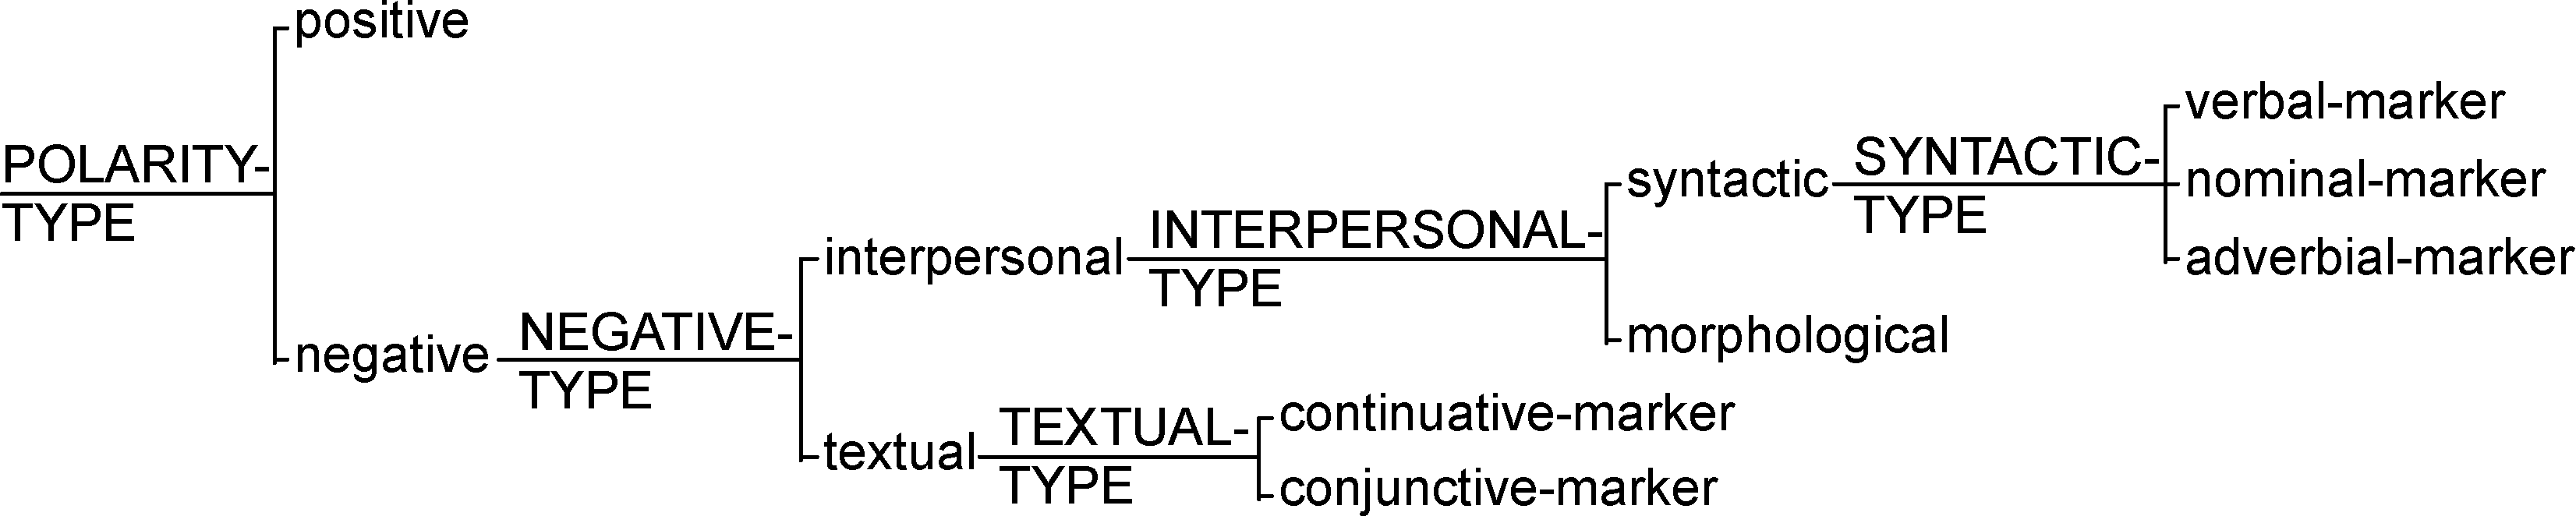
\includegraphics[width=\textwidth]{Figures/SFL-grammar/polarity-system.pdf}
    \caption{System network of POLARITY}
    \label{fig:polarity}
\end{figure}

But the activation relation among systems in the cline of delicacy is not always taxonomic. Another relation is ``enables selection of'' without any sub-categorisation implied. As an example see the FINITENESS system in Figure \ref{fig:finitness-fraction} where in case that the finite option is selected then what this choice enables is not subtypes of finite but merely other systems that become available i.e. DEIXIS and INDICATIVE TYPE. The latter is there because selection of finite implies also selection of indicative feature in a sibling of FINITNES system, MOOD-TYPE comprised of options indicative and imperative.

\begin{figure}[!ht]
    \centering
    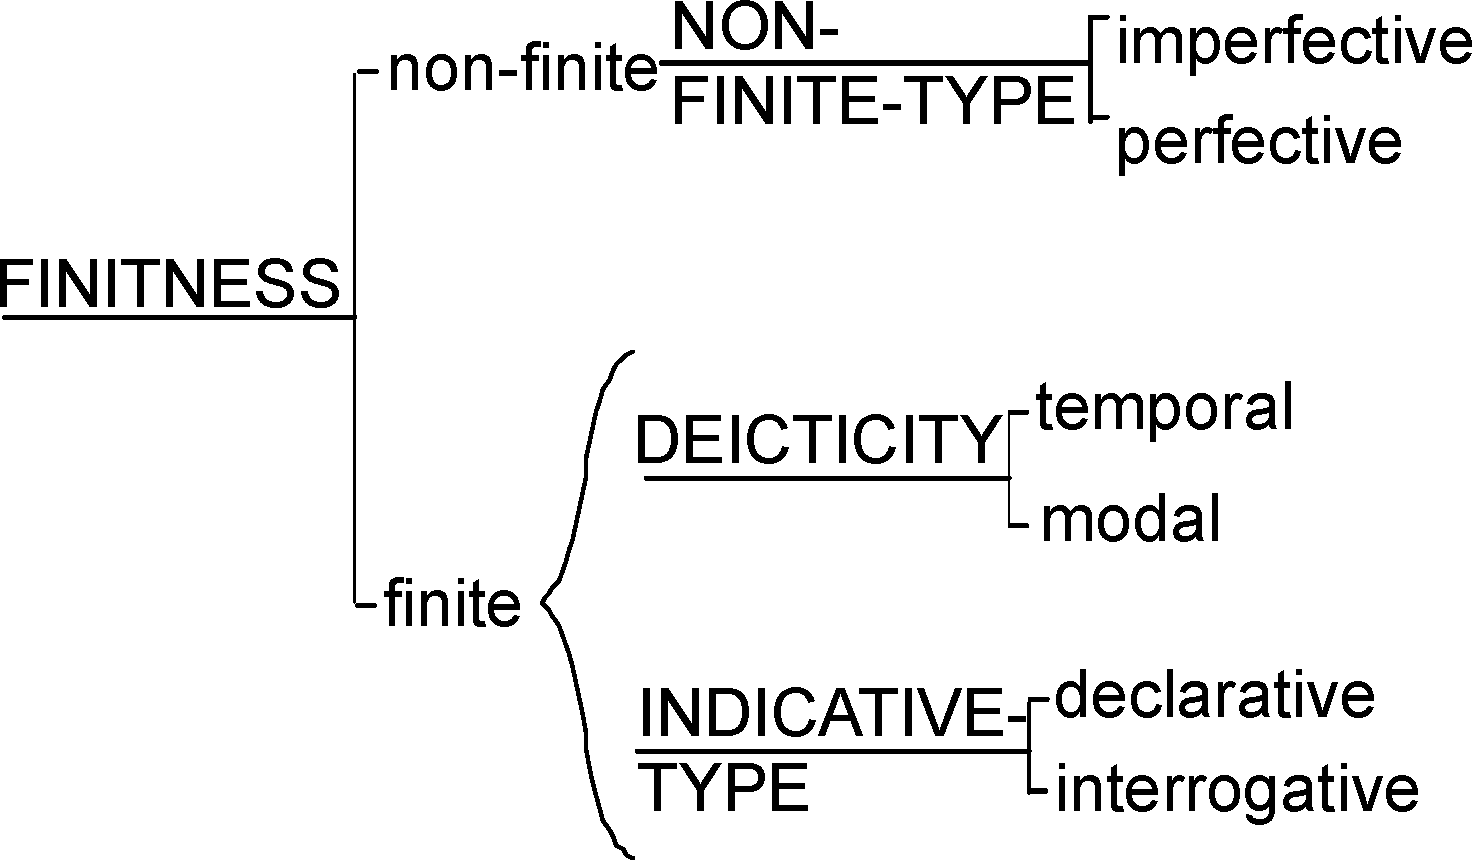
\includegraphics[width=0.5\textwidth]{Figures/SFL-grammar/finitness-system.pdf}
    \caption{A fraction of the finiteness system where increase of delicacy is not a ``is a'' relation}
    \label{fig:finitness-fraction}
\end{figure}

The distinction in the systemic relations is incorporated into the technical data structure definitions and traversal algorithms proposed in the Chapter \ref{ch:data-structures}.

\subsection{Unit classes}
\label{sec:unit-classes}
%Fawcett drops the concept of rank system (discussed in Section \ref{sec:rank-system}) and through a bottom-up approach redefining the class as a ``class of unit'' as in \ref{def:class2}.

In SFL at large there is the consensus that linguistic forms and meanings are intertwined and mutually determined just like for any sign in a Saussurean approach to language. Both Halliday (quote below) and Fawcett (Definition \ref{def:class2}) adopt this position. 

\begin{quotation}
	\dots something that is distinctly non-arbitrary [in language] is the way different kinds of meaning in language are expressed by different kinds of grammatical structure, as appears when linguistic structure is interpreted in functional terms \citep{Halliday2003-Ideas-about-language}.
\end{quotation}

When it comes to establishing the lexicogrammatical classes the two schools diverge. Halliday adopts the traditional grammar \textit{word classes} or \textit{parts of speech}: noun, verb, adjective etc. He then derives a set of groups (e.g. nominal group, verbal group, adverbial group etc.) that share properties of the word classes. In fact the class, in Halliday's words, ``indicates the in a general way its potential range of grammatical functions'' \citep[76]{Halliday2013}. For example the nominal group is a formation that functions as a noun may do and expresses same kind of meaning. 

Following the idea that major semantic classes of entities (situations, things, qualities and quantities) correspond to the major syntactic units, Fawcett decided to mirror them into the lexicogrammar. This lead to a semantically based classification of syntactic units: clause, nominal group, prepositional group, quality group and quantity group \citep[193--194]{Fawcett2000} along with a set of minor classes such as genitive and proper name clusters. This is, in a way, a tight coupling of the grammatical units with an ontology which may be subject to change in the future. The converse may also be stated that the traditional part of speech are disconnected from the semantics in the sense that there is no one to one correspondence (as Fawcett attempts) but rather complex set of mappings. Establishing the exact interface of syntax and semantics is a hot ongoing theoretical exploration across the entire linguistic discipline a difficult task in practice. This discussion however is beyond the scope here.   

In the current work I side with the Sydney classification of syntactic units that is close in line with traditional syntactic classifications \citep{Quirk1985}. I adopt the clause as a unit plus the four group classes of the Sidney grammar depicted in \mbox{Figure \ref{fig:group-classes}}. 

\begin{figure}[H]
	\centering
	\begin{subfigure}{.5\textwidth}
		\centering
		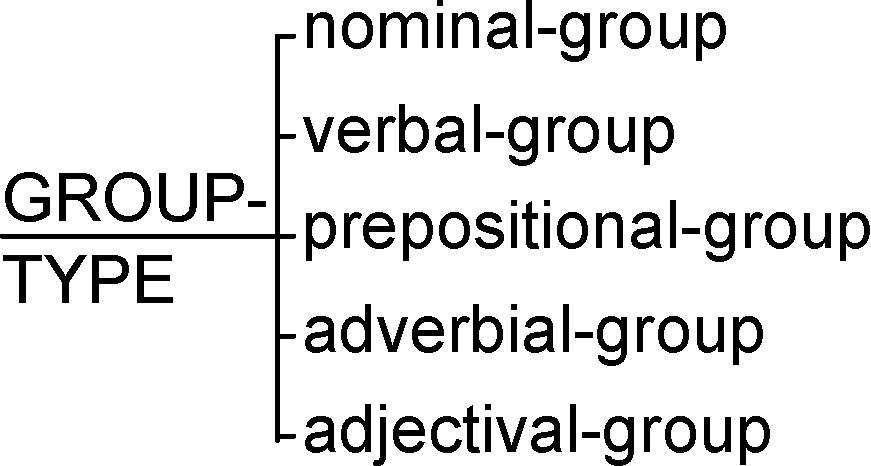
\includegraphics[width=0.57\linewidth]{Figures/SFL-grammar/group-classes.pdf}
		\caption{The group classes}
		\label{fig:group-classes-sub1}
	\end{subfigure}%
	\begin{subfigure}{.5\textwidth}
		\centering
		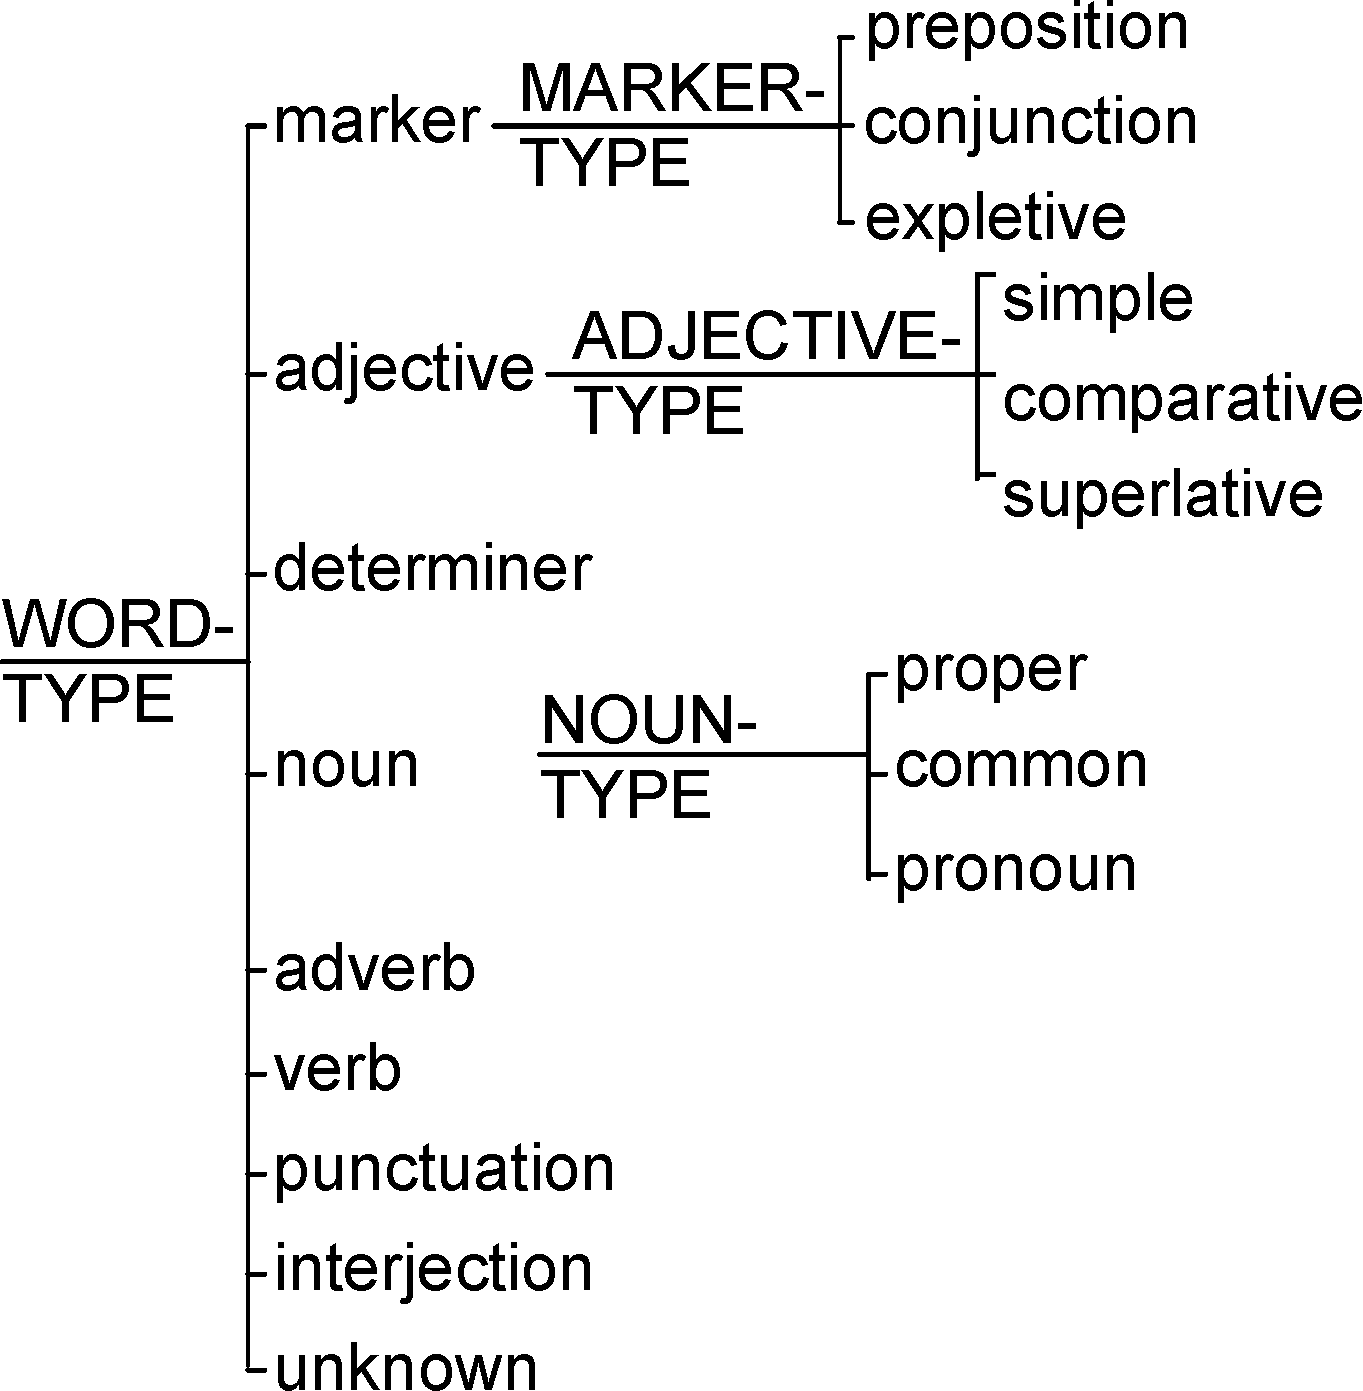
\includegraphics[width=0.9\linewidth]{Figures/SFL-grammar/word-classes.pdf}
		\caption{The word classes}
		\label{fig:group-classes-sub2}
	\end{subfigure}
	\caption{The group and word classes}
	\label{fig:group-classes}
\end{figure}

%The main reason is that Cardiff classes are beyond the syntactic variations of the grammar and blend into lexical semantics which makes it difficult to apply to parsing, at least nowadays with current state of word classification.

The word classes or part of speech tags that I adopt here are the ones employed to annotate Penn Treebank corpora called the Penn tag set \citep{Marcus1993} which, like Sidney unit classes, are also in line with the traditional grammar. This tag set has become a widely accepted standard in mainstream computational linguistics and there are multiple implementation of the part of speech taggers. The Stanford Parser which plays an important role in the software implementation of this thesis and is described in the Chapter \ref{ch:dependecy-grappamr}, employs precisely the Penn tag set.

The Penn tag set was developed to annotate the Penn Treebank corpora \citep{Marcus1993}. It is a large, richly articulated tag set that provides distinct codings for classes of words that have distinct grammatical behaviour.

The Penn tag set is based on the Brown Corpus tag set \citep{Kucera1968} but differs in several ways. First, the authors reduced the lexical and syntactic redundancy. In the Brown corpus there are many unique tags to a lexical item. In the Penn tag set the intention is to reduce this phenomenon to a minimum. Also distinctions that are recoverable from lexical variation of the same word such as verb or adjective forms or distinctions recoverable from syntactic structure are reduced to a single tag. 

Second the Penn Corpus takes into consideration the syntactic context. Thus the Penn tags, to a degree, encodes syntactic functions when possible. For example, \textit{one} is tagged as NN (singular common noun) when it is the head of the noun phrases rather than CD (cardinal number). 

Third, Penn POS set allows multiple tags per word, meaning that the annotators may be unsure of which one to choose in certain cases. There are 36 main POS and 12 other tags in the Penn tag set. A detailed description of the schema, the design principles and annotation guidelines are described in \citep{Santorini1990}. Figure \ref{fig:group-classes} depicts a classification summarising the Penn tag set. 



\subsection{Syntactic and semantic heads}
\label{sec:heads}
%TODO[JB]I fear this is confused. A grammatical head cannot be semantic, because it is grammar and not semantics: different strata. Do you mean that the grammatical heads may be *motivated* by semantic or syntactic criteria?
In SFG the heads may be motivated by semantic or syntactic criteria (simply called here semantic or syntactic heads). In most cases they coincide but there are exceptions when they differ or even diverge. This topic is especially important in the discussions of the \textbf{nominal group} structure (continued in Section \ref{sec:nominal-group}) on which \citet{Halliday2013} offers a thorough examination and \citet{Fawcett2000} provides a more generic perspective.

In this discussion I show few examples when the syntactic and semantic heads diverge and argue my position on the group formation on two points. First, the class of the Head (in Sydney school) or pivotal element (in Cardiff school) is not always raised to establish the group class but the whole underlying structure determines the group class. Second, that syntactically motivated heads are easy to establish because they are based solely on the formal grounds whereas the semantic heads require an evaluation at the level of entire group, once one is established, employing additional lexical semantic resources. This can be a two step process but in the current implementation only the group structure on syntactic grounds is provided. 

As mentioned before in Section \ref{sec:functions-metafunctions}, Sydney grammar fulfils the exhaustiveness principle (Generalization \ref{def:exhaustiveness}) through multiple parallel structures while Cardiff grammar through a single syntactic structure resembling a mixture of the former.

Let's briefly return to the Example \ref{ex:small-wooden} analysed with Sydney grammar in Table \ref{tab:example-substructure-analisys-logical} and \ref{tab:example-substructure-analisys} that reflect the nominal group logical and experiential structures \citet[391]{Halliday2013}. When the Head (called here the \textit{syntactic head} of the nominal group) coincides with the Thing (called here the \textit{semantic head}) we say that they are conflated (Definition \ref{def:conflation}) and examples as this one may lead to the assumption that the Head, which is motivated by syntactic criteria, is also always the Thing which is motivated by the semantic criteria, but this is not so.

The logical structure is a Head-Modifier structure and ``represents the generalised logical-semantic relations that are encoded in the natural language'' \citep[388]{Halliday2013}. The experiential structure of the nominal group as a whole has the function of specifying the class of things, through the Thing element, and some category of membership in this class, through the rest of the elements. In the nominal group there is always a Head but the Thing may be missing and so the Head element is conflated with either Epithet, Numerative, Classifier or Deictic instead.

\begin{exe}
	\ex\label{ex:one} (Have) a cup of tea. 
   	\ex\label{ex:the-old-example} The old shall pass first.
	\ex\label{ex:three} I'll give you three.
\end{exe}


%%TODO[JB] OK, got what you mean: but actually, in (Sydney) SFG, 'Head' is only a term of the logical metafunction, not of interpersonal *or* experiential. So the assumption that the Thing is automatically the Head is what is wrong here. One can see this is phrases such as:
%
%'I'll give you three'
%
%the Thing is not even there and the Head (logical) has shifted along to the numerative. So where do you get the idea that the Thing is necessarily the Head? If this is said somewhere give a reference (exact, with page numbers and possibly even with quotes: it is not enough, actually, to refer to entire books when you pursue a discussion, you should be giving the exact relevant page numbers).

Consider Example \ref{ex:one} analysed with Sydney and Cardiff grammars in Table \ref{tab:the-head-differences}. In the Sydney Grammar the semantic and the syntactic heads differ. In the experiential analysis the semantic head is ``tea'' which functions as Thing, while in the logical analysis the syntactic head is ``cup'' which functions as Head. Cardiff Grammar does not offer multi-structural analysis and there is no Head/Thing distinction. The functional elements are already established based on semantic criteria and this is further discussed in Section \ref{sec:nominal-group}. 

\begin{table}[!ht]
	\centering
	\begin{tabular}{|c|c|c|c|c|c|}
        \hline
        \multicolumn{2}{|c|}{\textit{}}                 & \textit{a}           & \textit{cup}         & \textit{of}         & tea          \\ \hline
        \multirow{2}{*}{Sidney Grammar} & experiential  & \multicolumn{3}{c|}{Numerative}                                   & Thing        \\ \cline{2-6} 
        & interpersonal & Pre-Modifier         & Head                 & \multicolumn{2}{c|}{Post-Modifier} \\ \hline
        \multicolumn{2}{|l|}{Cardiff Grammar}           & \multicolumn{2}{c|}{Quantifying Determiner} & Selector            & Head         \\ \hline
    \end{tabular}
	\caption{Analysis of Example \ref{ex:one} with Sydney and Cardiff grammars: diverging semantic and syntactic heads.}
	\label{tab:the-head-differences}
\end{table}

%%TODO[JB] is this all relevant for parsing: you should make the relevance of all these discussions for the purpose of parsing much clearer: at present this often goes under. (defined in Section \ref{sec:elements-of-structure})
In the nominal group ``The old'' which is Subject in Example \ref{ex:the-old-example}, the Head is adjective ``old'' and not a noun as would normally be expected. The noun modified by the adjective ``old'', also the \textit{pivotal element} of the group defined in Section \ref{sec:elements-of-structure}, is left covert and it should consequently be recoverable anaphorically or cataphorically from the context. We can insert a generic noun ``one'' to form a canonical noun group ``the old one''. In such cases when the pivotal noun is missing, the logical Head is conflated with other element in this case the Epithet. The group class is not raised from the word class to quality group but is identified by internal structure  of the whole group and in this case the presence of determiner signals a nominal class. Similarly, in Example \ref{ex:three}, ``three'' in Sydney grammar is a nominal group where the Thing is missing and the Head has shifted left towards the Numeral. With examples as these ones, Fawcett argues that none of the constituting elements of the unit is mandatorily realised, even the so called pivotal element which is the group defining element. In Chapter \ref{ch:gbt} is provided an in depth description of the recovering mechanisms for covert nominal elements at the level of the clause.

% In Cardiff terms the Head (also the pivotal element of the nominal group) is missing. In such cases the pivotal element is conditioner covert and can be filled by the impersonal pronoun ``one(s)'' that shall be anaphorically resolved in the discourse context. 
 

%\begin{table}[!ht]
%    \centering
%    \resizebox{\textwidth}{!}{%
%        \begin{tabular}{|c|c|c|c|c|c|}
%            \hline
%            & \textit{I}    & \textit{will}   & \textit{give}   & \textit{you}  & \textit{three} \\ \hline
%            \multirow{4}{*}{Sydney Grammar (interpersonal)}    & Subject       & Finite          & Predicator      & Complement    & Adjunct        \\ \cline{2-6} 
%            & nominal group & \multicolumn{2}{c|}{verbal group} & nominal group & nominal group  \\ \cline{2-6} 
%            & Thing         & Auxiliary       & Event           & Thing         & Numerative     \\ \cline{2-6} 
%            & pronoun       & modal verb      & verb            & pronoun       & numeral        \\ \hline
%            \multirow{2}{*}{Cardiff Grammar (syntax)} & Subject       & Operator        & Main Verb       & Complement    & Adjunct        \\ \cline{2-6} 
%            & pronoun       & modal verb      & verb            & pronoun       & numeral        \\ \hline
%        \end{tabular}%
%    }
%    \caption{My caption}
%    \label{tab:three-sydney}
%\end{table}


%TODO follow the argumentation along the promisses in the section introduction

In this work I adopt the principles for establishing the logical structure of Sydney Grammar. It resonates closely with the traditional ``semantically blinded'' grammars because and it always provides a Head element even if it differs from the syntactically motivated pivotal element in Cardiff Grammar. Moreover these logical Heads correspond to dependency heads established in the Stanford dependency parse. Chapter \ref{ch:dependecy-grappamr} provides the grounds for cross-theoretical mappings and the empirical evaluation in Chapter \ref{ch:evaluation} validates it.

In language is not unusual to have nominal groups with the Thing missing or elliptic clauses with the Main verb missing therefore no rigid correspondence can be established between the logical Head and unit class. 
%And because the unit class depends on its internal structure (in Cardiff school), this leads to a circular interdependency between the unit class and the unit structure. 
In this thesis the structure creation is performed in two steps first establishing the group boundaries and the unambiguous unit elements through a top down perspective (that is Sydney approach to unit creation) and second for each established group evaluate the internal structure in order to establish the group class (that is Cardiff approach to group formation). This process is detailed in the Chapter \ref{ch:parsing-algorithm}.

The evaluation in the second step, besides finalising the syntactically motivated unit structure, can as well assign semantically motivated unit structure. This part however is left out in the current thesis for the groups and only the clauses receive semantic role labels and process types described in Chapter \ref{ch:semantic-parsing}.

%To solve th issue Fawcett argues for a bottom-up approach where head-modifier relations are identified between lexical items and then between units (i.e. groups and clauses) serving as cues to identify elements of the higher unit and therefore its class. Usually the class membership of head is raised to the unit class although sometimes the presence or absence of certain elements (during the reconstruction process) may alter the unit class to a different one from the logical head.

%Based on the unit class, the logical structure heads are conflated with specific functions. For instance in nominal group the Head is usually conflated with the Thing, in quality group with the Apex, in quantity group with the Amount, in clause with the Main Verb and so on. 

%%TODO conclude
%Conclusion: 
%I use the Sydney approach to heads which is syntactically motivated, It is possible to convert to Cardiff semantic heads in a second step. Currently is not implemented and it is subject to future work. 


\subsection{Coordination as unit complexing} % coordination as
%TODO: the complex class is semantic and not grammatical
%TODO: sometimes the second element is more representative of the complex or the first one maybe, maybe just take the class of the first unit and then ingnore teh class of the rest, or the last one and ingnore classes of the first ones
\label{sec:coordination}

In Sydney Grammar unit complexes fill an important part of the grammar along with the \textit{taxis relations} (Definition \ref{def:taxis}) which express the interdependency relations in unit complexes. \textit{Parataxis} relations bind units of equal status while the \textit{Hypotaxis} ones bind the dominant and the dependant units. Fawcett bypasses the taxis relations replacing them with coordination and embedding \citep[271]{Fawcett2000} leading to abandonment of unit complexing entirely. While embedding elegantly accounts for the depth and complexity of syntax, this approach to coordination is problematic.

Hereafter I discuss the utility and even necessity of keeping unit complexes in parsing. In particular I address the treatment of group and clause \textit{coordination} but the same
principle applies to fixed idiomatic structures such as \textit{comparatives}, \textit{conditionals} or \textit{appositions}.

Treatment of the coordination phenomena is a challenge not only for SFL but for other linguistic theories as well. Sydney Grammar approaches it through unit complexing and taxis relations while Cardiff Grammar treats this phenomena as multiple distinct units filling or expounding the same element. 

%Sydney
%%TODO the function of the conjunction is not very clear, with the logical accounts

Table \ref{ex:Sydeny-example-analisys} illustrates an example analysis where the Complement is filled by a homogeneous nominal group complex held together through \textit{paratactic extension} where the first element is a nominal group and the second is nominal group together with the conjunction which is not part of the experiential structure but remains accounted only in the logical structure of the nexus. 

\begin{table}[h]
    \centering
    \begin{tabular}{cc|c|c|c|c|c|}
        \hline
        \multicolumn{1}{|c|}{\textit{Ike}} & \textit{washed} & \textit{his} & \textit{shirt} & \textit{and} & \textit{his} & \textit{jeans} \\ \hline
        \multicolumn{1}{|c|}{Subject} & Predicate/Finite & \multicolumn{5}{c|}{Complement} \\ \hline
        &  & \multicolumn{2}{c|}{1} & \multicolumn{3}{c|}{+2} \\ \cline{3-7} 
        &  & Deictic & Thing &  & Deictic & Thing \\ \cline{3-4} \cline{6-7} 
    \end{tabular}
    \caption{Clause with nominal group complex}
    \label{ex:Sydeny-example-analisys}
\end{table}

In Table \ref{tab:sydney-coordination-ifg} the Epithet is filled by a nexus of paratactic extension. The first element of the nexus is the word ``immediate'' and the second element is the set of words ``and not so far distant''. The ``not so far distant'' is an adverbial group with a logical structure of sub-modifiers already discussed in Section \ref{sec:rank-system} and the conjunction ``and'' is left implicitly part of the logical structure of the nexus creating a gap in the structure that is addressed in this discussion. Also note that, in Sydney Grammar the coordination is accounted as unit complex ensuring that only one unit fills an element of the parent, in contrast, as we will see below, to Cardiff Grammar. 

\begin{table}[H]
    \centering
%    \resizebox{\textwidth}{!}{%
        \begin{tabular}{ccc|c|c|c|c|c}
            \hline
            \multicolumn{1}{|c|}{\textit{the}} & \multicolumn{1}{c|}{\textit{immediate}} & \textit{and}          & \textit{not} & \textit{so} & \textit{far} & \textit{distant}          & \multicolumn{1}{c|}{\textit{future}} \\ \hline
            \multicolumn{7}{|c|}{Modifier} & \multicolumn{1}{c|}{Head} \\ \hline
            \multicolumn{1}{|c|}{$\gamma$}            & \multicolumn{6}{c|}{$\beta$}                                                                                                                  & \multicolumn{1}{c|}{$\alpha$}               \\ \hline
            \multicolumn{1}{|c|}{Deictic}      & \multicolumn{6}{c|}{Epithet}                                                                                                            & \multicolumn{1}{c|}{Thing}           \\ \hline
            \multicolumn{1}{c|}{}              & \multicolumn{1}{c|}{1}                  & \multicolumn{5}{c|}{+2}                                                                       &                                      \\ \cline{2-7}
            \multicolumn{1}{l}{} & \multicolumn{1}{l}{} & \multicolumn{1}{l|}{} & \multicolumn{3}{c|}{Sub-Modifier} & Sub-Head & \multicolumn{1}{l}{} \\ \cline{4-7}
            &  &  & $\delta$ & $\gamma$ & $\beta$ & $\alpha$ &  \\ \cline{4-7}
        \end{tabular}%
%    }
    \caption{Nominal group with word complex from \citep[564]{Halliday2013}}
    \label{tab:sydney-coordination-ifg}
\end{table}

%Cardiff
%%TODO the filling of an element with a conjunction is not right, 
%%TODO conjunction element should be outside the group
%TODO first group/word can be the head and the rest modifier or the conjunction can be head and the others modifier, but both are tricky, how about apposition? 

In Table \ref{ex:Cardiff-example-analisys} is presented an example of analysis with Cardiff Grammar. The Complement is filled by two \textit{sibling} nominal groups ``his shirt'' and ``and his jeans'' that are both of them fill the same element in accordance to Definition ref{def:coordination}. The conjunction ``and'' is accounted directly as part of the nominal group structure.

\begin{table}[!ht]
	\centering
        \begin{tabular}{cc|c|c|c|c|c|}
            \hline
            \multicolumn{1}{|c|}{\textit{Ike}} & \textit{washed} & \textit{his}       & \textit{shirt} & \textit{and} & \textit{his}       & \textit{jeans} \\ \hline
            \multicolumn{1}{|c|}{Subject}      & Main Verb       & \multicolumn{5}{c|}{Complement}                                                          \\ \hline
             &  & Deictic Determiner & Head & \& & Deictic Determiner & Head \\ \cline{3-7} 
        \end{tabular}%
	\caption{Coordination analysis in Cardiff Grammar}
	\label{ex:Cardiff-example-analisys}
\end{table}

Opinions are divided (between Sydney and Cardiff schools) whether to invite the notion of a complex unit to handle coordination or not. If we side with Cardiff grammar and dismiss the unit complex then we allow an element to be filled by more than one units. And this is a problem because if we do not account unit elements each in a unique place within the unit structure then we loose the capacity to order them. Therefore in this thesis I adopt the Sydney definition of structure (Definition \ref{def:structure}) that constraints each element into a single place that is filled by another unit. Therefore the conjunction must be a nexus acting as a single unit filling a single element. 

I argue for adoption of such unit type in order to ensure that maximum one unit can fill the place of an element. In the theory of grammar, only units are accounted for structure while the elements can only be filled by an unit (see Figure \ref{fig:structure-representation}). Allowing multiple units to fill an element requires accounting at least for the \textit{order} if not also for the relation between the filler units. The structure as it is described in theories of grammar by Halliday \citep{Halliday2002} and Fawcett \citep{Fawcett2000} is defined by the unit and not the element. There is no direct reference in the theory to the unit ordering. Instead, the order relation is accounted in the structure through the concept of place. A unit has a specific possible structure in terms of places of elements which hold absolute position in the unit structure or relative one to each other. Therefore if an element is filled by two units simultaneously it constitutes a violation of the above principle as the order of those units is not accounted for but it matters which is easy to show in the following examples.

\begin{exe}
	\ex\label{ex:conj2-extra-marker1}
	(Both my wife and her friend) arrived late.  
	\ex\label{ex:conj2-extra-marker11} * (And her friend both my wife) arrived late.
	\ex\label{ex:conj2-extra-marker2}
	I want the front wall (either in blue or in green). 
	\ex\label{ex:conj2-extra-marker21}
	* I want the front wall (or in green either in blue). 
\end{exe}

If the order would not have mattered then we could say that the conjunctions from the example \ref{ex:conj2-extra-marker1} can be reformulated into \ref{ex:conj2-extra-marker11} and the one from \ref{ex:conj2-extra-marker2} into \ref{ex:conj2-extra-marker21}. But such reformulations are grammatically incorrect. Obviously the places do matter and they need to be accounted in the unit structure as one element per place with no more than a single unit filling it.

I turn now to the role and position of lexical items signalling the conjunction which I consider having no place in the structure of the conjuncted units but outside of them, that way forming together a higher order unit, the \textit{complex unit}. This is contrary to what is being described in Cardiff and Sydney grammars for different reasons. 

Fawcett present the Linker elements (\&) which are filled by conjunctions as parts of virtually any unit class placed in the first position of the unit. For example in the ``or in green'' the presence of ``or'' signals the presence at least of one more unit of the same nature and does not contribute to the meaning of the prepositional group but to the meaning outside the group requiring presence of a sibling. Even more, the lack of a sibling most of the time would constitute an ungrammatical formulation. The only potential objection here is for the perfectly acceptable cases of clauses/sentences starting with a conjunction such as ``and'' or ``but''. In those cases the conjunction plays a textual function and still invites the presence of a sibling clause/sentence preceding the current one to be resolved in a clause complex or discourse level. 

Halliday omits to discuss in IFG \citep{Halliday2013} the place of Linkers. He implicitly proposes the same as Fawcett through his examples of paratactic relations at various rank levels \citep[422, 534, 564, 566]{Halliday2013} that the lexical items signalling conjunction are included in the units they precede in the logical structure but not the experiential one. The main insufficiency here is that the logical structure does not provide any meaningful elements or unit class but some sort of proto-elements that resemble rather places than any functions. In this sense I consider treatment of conjunctions insufficiently accounted in IFG.  

So conjunctions and pre-conjunctions shall not be placed inside the conjuncted units because they do not contribute to their meaning. They shall be enclosed as Linkers into unit complexes. But if we adopt the unit complexing then we need to define a unit structure. Hence I propose the following generic structure for the \textit{coordination unit}.

\begin{table}[!h]
    \centering
    \begin{tabular}{|c|c|c|c|c|}
        \hline
        Pre-Linker & Initiating Conjunct & ... Conjunct ... & Linker & Conjunct \\ \hline
        \multicolumn{2}{|c|}{1} & + 2 ... + n_{-1} & \multicolumn{2}{c|}{+ n} \\ \hline
    \end{tabular}
    \caption{Generic structure of the coordination unit}
    \label{tab:coordination-complex}
\end{table}

In Table \ref{tab:coordination-complex} the first row presents a series of Conjuncts where the first one is initiating or the head and the rest are continuation Conjuncts of the former. In the first place there may be a Pre-Linker element such as ``both'' or ``either'' for example but it is optional and in the place before the last one is located the Linker element that determines the type of coordination. On the second row I provide, for orientation purposes, the Sydney logical structure of a paratactic expansion applied to the coordination unit complex. Note that the Pre-Linker and the Linker elements are merged with the conjuncted units.

Applying this structure to the previous example yields analysis such as in Table \ref{tab:distant-future-compelx}. The nominal group has the Epithet element filled by a coordination group formed of two Conjuncts and a Linker.

\begin{table}[H]
    \centering
    \begin{tabular}{c|c|c|c|c|c|c|c}
        \hline
        \multicolumn{1}{|c|}{\textit{the}} & \textit{immediate} & \textit{and} & \textit{not} & \textit{so} & \textit{far} & \textit{distant} & \multicolumn{1}{c|}{\textit{future}} \\ \hline
        \multicolumn{1}{|c|}{Determiner} & \multicolumn{6}{c|}{Epithet} & \multicolumn{1}{c|}{Head} \\ \hline
        & Initiating Conjunct & Linker & \multicolumn{4}{c|}{Conjunct} &  \\ \cline{2-7}
    \end{tabular}
    \caption{Example analysis with coordination unit complex structure}
    \label{tab:distant-future-compelx}
\end{table}

Adopting the unit complex and in particular coordination unit requires two more clarifications (1) does the complex unit carry a syntactic class, and if so according to which criteria is it established? (2) Does it have any intrinsic features or all of them are inherited from the conjuncts?

Zhang states in her thesis that the coordinating constructions do not have any categorial features thus there is no need to provide a new unit type. Instead the categorial properties of the conjuncts are transferred upwards \citep{NinaZhang2010}. For example if two nominal groups are conjuncted then the complex receives the nominal class.  

This principle holds for most of the cases however there are rare cases when the units are of different classes. Consider \ref{ex:conj3-different-unit-types} analysed in Table \ref{tab:mixed-coordination} where the conjuncts are a nominal group ``last Monday'' and a prepositional group ``during the previous weekend''.

\begin{exe}
	\ex\label{ex:conj3-different-unit-types}
	I lost it (either last Monday or during the previous weekend). 
\end{exe}

\begin{table}[H]
    \centering
    \begin{tabular}{|c|c|c|c|c|c|c|c|}
        \hline
        \textit{either} & \textit{last} & \textit{Monday} & \textit{or} & \textit{during} & \textit{the} & \textit{previous} & \textit{weekend} \\ \hline
        Pre-Linker & \multicolumn{2}{c|}{Initiating Conjunct} & Linker & \multicolumn{4}{c|}{Conjunct} \\ \hline
    \end{tabular}
    \caption{Coordination group with mixed class conjuncts}
    \label{tab:mixed-coordination}
\end{table}

%In unit types are of different classes: a nominal group and a prepositional phrase.
In this case there are two unit types that can be raised and it is not clear how to resolve this case. Options are (a) to leave the generic class \textit{coordination complex}, (b) transfer the class of the first unit upwards, or (c) semantically resolve the class as both represent temporal circumstances even if they are realised through two different syntactic categories. This means that if no sub-classification is provided based on the constituent units below than there is no need to project/transfer upward the class of the conjunct units. In this work I decided to leave the class generic and leave for the future an extensive unit complex classification.

I turn now to the last issue of this discussion, specifically whether the complex unit may have intrinsic features emerging from the conjunct elements. 

In the example \ref{ex:conj-plural-right} the conjunction of two singular noun groups requires plural agreement with the verb. Even though semantic interpretation that only one item is selected at a time, syntactically both items are listed in the clause and attempting third person singular verb forms in \ref{ex:conj-plural-wrong} is grammatically incorrect. That leads to the conclusion that the coordination complex can have categorial features which none of the constituting units has. 

\begin{exe}
	\ex\label{ex:conj-plural-right}
	A pencil or a pen \textbf{are} equally good as a smart-phone.
	%\ex\label{ex:conj-plural-right1} A fork and knife \textit{have} to be placed on the sides of each plate.
	\ex\label{ex:conj-plural-wrong} * A pencil or a pen \textbf{is} equally good as a smart-phone.
	%\ex\label{ex:conj-plural-wrong1} * A fork and knife \textit{has} to be placed on the sides of each plate.
\end{exe}

\begin{figure}[!h]
	\centering
	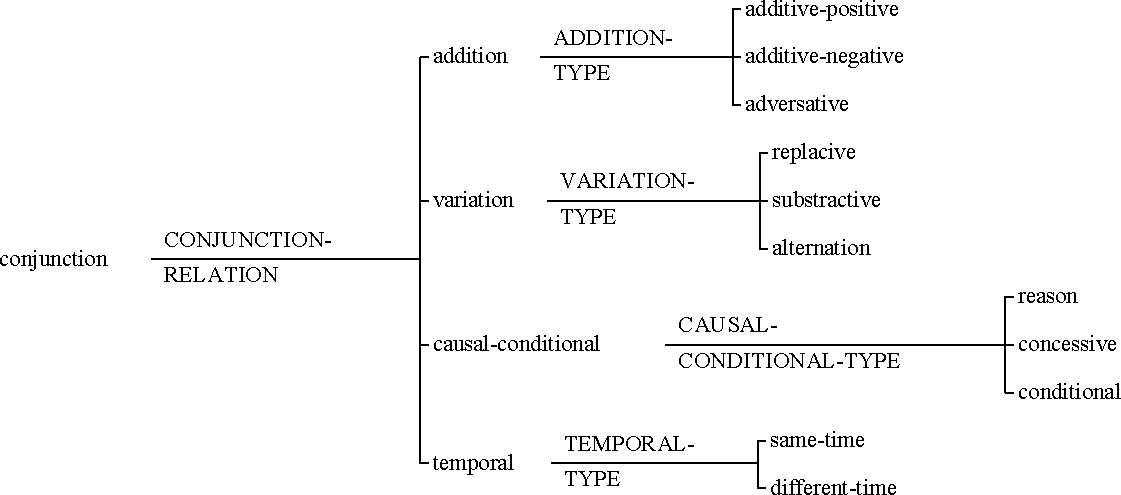
\includegraphics[width=\textwidth]{Figures/SFL-grammar/conjunction-system.pdf}
	\caption{Systemic network of coordination types}
	\label{fig:conj-rel-types}
\end{figure}

In the case of nominal group conjunction we can see that the plural feature emerges even if each individual unit is singular. For other unit classes it is not so obvious whether there are any linguistic features that emerge at the conjunction level. The meaning variation is semantic as for example conjunction of two verbs or clauses might mean very different things such as consecutive actions, concomitant actions or presence of two states at the same time and so on. This brings us to another feature of the coordination complex - the type of the relationship it constructs. The lexical items expounding the Linker and Pre-Linker (e.g. \textit{and}, \textit{or}, \textit{but}, \textit{yet}, \textit{for}, \textit{nor} or \textit{so}) are indicator of relationship among the conjuncts and together can be systematised as the relationship types in the systemic network in \mbox{Figure \ref{fig:conj-rel-types}}.

%The coordination complex has a structure as depicted in figure \ref{fig:coord-complex-elements}. The lexical item signalling the coordination complex is the head of the construction. The Conjunct elements are the ones being related to each other and they can be filled or expounded by virtually any unit type. The Enumerator element substitutes the head and delimits the Conjuncts when there are more than two of them. The Enumerator is almost always a comma in written texts. 

%Adopting the unit complexing enables various kinds of constructions and coordination is only one of them. Below we discuss taxis relations and their role in unit complexing.

This section laid out how and why I treat the coordination phenomena in parsing. I adopt the unit complexing mechanism with taxis relations described in Sydney grammar in order to account for a new unit class, the \textit{coordination unit}. I do that to ensure that each element of a unit is filled by no more than one other unit contrary to what Cardiff grammar proposes (see Definition \ref{def:coordination}). But taxis relations in Sydney grammars are represented via logical structures which is not rich enough to account for internal structure of the coordination unit. Therefore I also propose here a unit structure in terms of ordered functional elements just as for the rest of unit classes. 
%This discussion aimed to solve the specifics of the coordination phenomena but in part it is generic enough to be applied to other unit complex types especially the ones with a fixes idiomatic structure such as comparatives, conditionals and so on. 
%I turn now to briefly discuss the units of

\section{The grammatical units for parsing}
\label{sec:discussion-unit-classes}

Now that the important theoretical details have been covered I would like focus on the specific grammars of the two schools. They have common parts and also differ in large parts on their paradigmatic and syntagmatic descriptions. This section discusses the main units considered in each of the grammars. As in the previous section I argue on pragmatic grounds for the adoption of unit structures from one or the other grammar. The argument runs along the lines that some unit structures are closer to the traditional syntactic analysis and thus are easier to detect and parse and the other ones may be a level of abstraction higher falling more on semantic grounds and thus becoming more difficult to capture in structural variance and requiring lexico-semantic resources.

%For the reasons of limited space I skipped introducing the Sydney and Cardiff grammars and in turn assume that the reader is familiar with the details fo both of them. And for a general overview of the unit structure in each of the grammars please refer to Appendix \ref{ch:syntax-overview}. 
%Nevertheless, as it is a parallel contrastive discussion, even if the reader is familiar with one grammar only I hope it becomes clear how does certain phenomena are dealt with in the other one. 

\subsection{Verbal group and clause boundaries}
\label{sec:verbal-grpoup-and-clause-division}
In Sydney Grammar the verbal group is described as an expansion of a verb just like the nominal group is the expansion of the noun\citep[396]{Halliday2013}. There are certainly words that are closely related and syntactically dependent on the verb all together forming a unit that functions as a whole. For example the auxiliary verbs, adverbs or the negation particles are words that are directly linked to a lexical verb. The verb group functions as Finite + Predicator elements of the clause in Mood structure and as Process in Transitivity structure. 

In Cardiff Grammar the verb group is dissolved moving the Main Verb as the pivotal element of the Clause unit. All the elements that form the clause structure and those that form the verb group structure are brought up together to the same level as elements of a clause. The clause structure in Cardiff Grammar comprises elements with clause related functions(like Subject, Adjunct, Complement etc.) and other elements with Main Verb related functions(Auxiliary, Negation particle, Finite operator etc.).

Regarded from the Hallidayan rank scale perspective, merging the elements of the verb group into clause structure is not permitted because the units are at different ranks. However it is not a problem for the relaxed rank scale version presented in subsection \ref{sec:rank-system}. The reason for adopting such an approach is best illustrated via complex verb groups with more than one non-auxiliary verb such as in examples \ref{ex:complex-verb-groups1}--\ref{ex:complex-verb-groups3}. 

I begin by addressing the impact of this merger on (a) the clause structure (b) the clause boundaries and (c) semantic role distribution within the clause.

\begin{exe}
	\ex\label{ex:complex-verb-groups1}
	(The commission \textbf{started to investigate} two cases of overfishing in Norway.)  
	\ex\label{ex:complex-verb-groups2}
	(The commission \textbf{started} (\textbf{to investigate} two cases of overfishing in Norway.))
	\ex\label{ex:complex-verb-groups3}
	(The commission \textbf{started} (\textbf{to finish} (\textbf{investigating} two cases of overfishing in Norway.)))
\end{exe}

%Then answers to the above questions boil down to whether we allow for more than one lexical verb per predicate or not. 
In Sydney Grammar ``started to investigate'' (in \ref{ex:complex-verb-groups1}) is considered a single predicate of investigation which has specified the aspect of event incipiency despite the fact that there are two lexical verbs within the same verbal group. The ``starting'' doesn't constitute any kind of process in semantic terms but rather specifies aspectual information about the investigation process. 
This is argued by looking at the conditions on the participants and it is equivalent in a formal approach to looking at where the selection restrictions for complements come from.
The boundaries of the clause governed by this predicate stretch to the entire sentence.

Semantically it is a sound approach because despite the presence of two lexical verbs there is only one event. However allowing such compositions leads to unwanted syntactic analysis for multiple lexical verb cases in examples such as \ref{ex:complex-verb-groups3}. To solve this kind of problem Fawcett dismisses the verb groups and merges their elements into clause structure. He proposes the syntactically elegant principle of \textit{one main verb per clause} \citep{Fawcett2008}. Applying this principle to the same sentence yields a structure of two clauses illustrated in example \ref{ex:complex-verb-groups2} where the main clause is governed by the verb ``to start'' and the embedded one by the verb ``to investigate''. Note the conflict between ``one main verb per clause'' with Halliday's principle that only whole units form the constituency of others (the (c) principle of rank scale described in subsection \ref{sec:rank-system}). So allowing incomplete groups into the constituency structure would breach the entire idea of unit based constituency. 

Semantically the clause in SFL is a description of an event or situation as a figure with a process, participants and eventually circumstances where the process is realised through a lexical verb. Looking back to our examples, does the verb ``to start'' really describes a process or merely an aspect of it? Halliday treats such verbs as aspectual and when co-occurring with other lexical verbs they are considered to form a single predicate. Accommodating Fawcett's stance, mentioned above and contradicting Halliday's approach, requires weakening the semantic requirement and allowing aspectual verbs to form clauses that contribute \textit{aspectually or modally} to the embedded ones. I mention also the modal contribution because some verbs like \textit{want, wish, hope} and others behave syntactically like the aspectual ones. Moreover, Fawcett introduces into the Cardiff Grammar Transitivity network an \textit{influential} process type including all categories of meanings that semantically function as process modifiers: tentative, failing, starting, ending etc.

I adopt here Fawcett's ``one main verb per clause'' principle which as a consequence changes the way clauses are partitioned, leads to abolition of the verbal group and introduces the ``influential'' process type. Next I discuss it's impact on the structure of the clause unit. 

\subsection{The Clause}
\label{sec:cardiff-clause}
It is commonly agreed in linguistic communities that the unit of the clause is one of the core elements in human language. 
%It is considered the syntactic unit that expresses semantic units of a situation referring to a potentially rich array of meanings. The clause structure has been studied for long time and 
The main clause constituents are roughly the same in SFL as the ones in the traditional grammar \citep{Quirk1985}, transformational grammar \citep{Chomsky1957} an indirectly in dependency grammar \citep{Hudson2010}.

In current work I adopt the Cardiff Grammar clause structure with the \textit{Main Verb} as pivotal element. Though there is no element that is obligatorily realised in English, I consider in the current work, the Main Verb to be way to flag a clause. In SFL are described clauses without a main verb such as minor clauses (exclamations, calls, greetings and alarms) that occur in conversational contexts and elliptical clauses \citet{Halliday2013} such as the one in example \ref{ex:elipted-clause}, none of which are covered in the present work.

\begin{exe}
	\ex\label{ex:elipted-clause} They were in the bar, \textit{Dave in the restroom and Sarah by the bar}.
\end{exe}

%As mentioned before in Definition \ref{def:structure} the elements of a structure are defined in terms of their function contributing to the formation of the whole unit.
I adopt Cardiff Grammar clause structure for English. It is formed of the \textit{Subject}, \textit{Finite}, \textit{Main Verb}, up to two \textit{Complements} and a various number of \textit{Adjuncts}. All the elements of the assumed verbal group are part of the clause as well such as Auxiliary Verbs, Main Verb Extensions, Negators etc. (see Appendix \ref{ch:syntax-overview} for a 
complete list).

%%TODO insert the complete list as done for nominal group below

%\todo*{}{TODO continue, maybe mention about the clause complexing}
%SFG accounts for how clauses form nexuses of tactic relations (see Definition \ref{def:taxis}).


\subsection{The Nominal Group}
\label{sec:nominal-group}

The nominal group expresses things, classes of things or a selection of instances in that class. This section argues for adoption of the Sydney grammar noun group structure with a specific extension. It is that the elements of the nominal group can be filled, in addition to word classes, by the groups as well. This possibility is opened by the rank scale relaxation (Section \ref{sec:rank-system}) and Cardiff embedding principle (Definition \ref{def:embedding}). In addition to that I argue below for working on semantic and syntactic heads in two steps. First create the structure with the syntactic one (the Head) and then derive the semantic one (the Thing).

\begin{table}[!ht]
    \centering
	\begin{tabular}{|c|c|c|c|c|c|}
		\hline
		\textit{those} & \textit{two} & \textit{old} & \textit{electric} & \textit{trains} & \textit{from Luxembourg} \\ \hline
		\multicolumn{4}{|c|}{Pre-Modifier}                               & Head            & Post-Modifier            \\ \hline
		Deictic        & Numerative   & Epithet      & Classifier        & Thing           & Qualifyier               \\ \hline
		determiner     & numeral      & adjective    & adjective         & noun            & prepositional phrase     \\ \hline
	\end{tabular}
	\caption{An example of a nominal group in the Sydney Grammar \citep[264]{Halliday2013}}
	\label{tab:example-ng}
\end{table}

In  Table \ref{tab:example-ng} an example analysis is presented of the nominal group proposed in the Sydney grammar \citep[364--369]{Halliday2013}. The Sydney nominal group is constituted by a head nominal item modified by descriptors or selectors such as: \textit{Deictic}, \textit{Numerative}, \textit{Epithet}, \textit{Classifier}, \textit{Thing} and \textit{Qualifier}. Each element has a fairly stable correspondence to the word classes, expected to be expounded by lexical items. Table \ref{tab:function-pos-mapping} presents the mappings between the elements of nominal group and the word classes. 

\begin{table}[h]
        \centering
	\begin{tabulary}{0.9\linewidth}{|C|C|}
		\hline
		\textbf{Experiential function in noun group} & \textbf{class (of word or unit)} \\ \hline
		Deictic                             & determiner, predeterminer, pronoun, adjective \\ \hline
		Numerative                          & numeral(ordinal or cardinal) \\ \hline
		Epithet                             & adjective \\ \hline
		Classifier                          & adjective, noun \\ \hline
		Thing                               & noun                         \\ \hline
		Qualifier                           & prepositional phrase, clause \\ \hline
	\end{tabulary}
	\caption{Mapping of noun group elements to classes \citep[379]{Halliday2013}}
	\label{tab:function-pos-mapping}
\end{table}

Inspired from Cardiff grammar, in addition to word classes, the elements of the nominal group can also be filled by the group classes corresponding to each word class above. This way the Numerative, in addition to words, can be filled by a noun group, Epithet by an adjectival group, Classifier by an adjective or noun group and finally each of the elements can be filled by a coordination group discussed in Section \ref{sec:coordination}.

%There is little variation in how these functions are linked to the word classes. However the variation is not provided in the Sydney Grammar as it is in Cardiff Grammar. The latter provides data driven filling probabilities for each functional element to a set of possible unit classes \citep{Fawcett2000}.

The elements in Cardiff Grammar differ from those of Sydney Grammar. Table \ref{tab:carfiff-ng} exemplifies a noun group analysed with Cardiff Grammar covering all the possible elements. Table \ref{tab:cg-mappings} provides a legend for the Cardiff Grammar acronyms along with mappings to unit and word classes that can fill each element.

\begin{table}[H]
	\resizebox{\linewidth}{!}{
		\begin{tabular}{|c|c|c|c|c|c|c|c|c|c|c|c|c|c|c|}
			\hline
			\textit{or} & \textit{a photo} & \textit{of} & \textit{part} & \textit{of} & \textit{one} & \textit{of} & \textit{the best} & \textit{of} & \textit{the} & \textit{fine} & \textit{new} & \textit{taxis} & \textit{in Kew} & \textit{,} \\ \hline
			\multicolumn{12}{|c|}{pre-modifiers} & head & \multicolumn{2}{c|}{post-modifiers} \\ \hline
			\& & rd & v & pd & v & qd & v & sd or od & v & dd & m & m & h & q & e \\ \hline
		\end{tabular}}
		\caption{The example of a nominal group in Cardiff Grammar}
		\label{tab:carfiff-ng}
	\end{table}
	%
	\begin{table}[h]
		\begin{tabulary}{\textwidth}{|C|C|C|}
			\hline
			\textbf{symbol} & \textbf{function meaning} & \textbf{class (of word or unit)} \\ \hline
			rd & representational determiner & noun, noun group \\ \hline
			v & selector ``of'' & preposition \\ \hline
			pd & partitive determiner & noun, noun group \\ \hline
			fd & fractional determiner & noun, noun group, quantity group \\ \hline
			qd & quantifying determiner & noun, noun group, quantity group \\ \hline
			sd & superlative determiner & noun, noun group, quality group, quantity group \\ \hline
			od & ordinative determiner & noun, noun group, quality group \\ \hline
			td & tipic determiner & noun, noun group \\ \hline
			dd & deictic determiner & determiner, pronoun, genitive cluster \\ \hline
			m & modifier & adjective, noun, quality group, genitive cluster \\ \hline
			h & head & noun, genitive cluster \\ \hline
			q & qualifier & prepositional phrase, clause \\ \hline
			\& & linker & conjunction \\ \hline
			e & ender & punctuation mark \\ \hline
		\end{tabulary}
		\caption{The mapping of noun group elements to classes in Cardiff grammar}
		\label{tab:cg-mappings}
	\end{table}
	%
	
The elements in Cardiff Grammar are based on semantic criteria supported by lexical and syntactic choices. Consequently some elements cannot be derived based on solely syntactic criteria, requiring semantically motivated lexical resources. Semantically bound elements which are a challenge are predominantly determiners \textit{Representational, Partitive, Fractional, Superlative, Typic Determiners} while the rest of the elements: \textit{Head, Qualifier, Selector, Modifier and Deictic, Ordinative and Quantifying Determiners} can be determined solely on the syntactic criteria. The latter correspond fairly well to the Sydney version of nominal group which is adopted in the present work with the benefits of the relaxed rank system replacing the sub-structures with embedded units and simplifying the syntactic structures. 
	
	%3. introduction of negation element, linker, punctuation
	%``No'' as determiner. negative pronoun noone.
	%\citep[62,109,185]{Quirk1985}, \citep[365--374]{Halliday2013}, 
	%
	%The negation element is in Cardiff Grammar in clause structure so that it is separated from the finite. It's adoption in noun structure might or might not be a good idea. It is useful for complex groups. 
	%
	%\begin{exe}
	%\ex \label{ex:example-of-no}
	%No breathing man or animal can escape that forest alive.
	%\end{exe} 
	
Another simplification is renouncing to distinction between the Head and Thing \citep[390--396]{Halliday2013} discussed in Section \ref{sec:heads}. Thus if the logical Head of the nominal group is a noun then it is labelled as the Thing leaving the semantic discernment as a secondary process and out of the current scope. Otherwise, in cases of nominal groups without the Thing element, if the Head is a pronoun (other than personal), numeral or adjective (mainly superlatives) then they function as Deictic, Numerative or Epithet. So, as will be described in Chapter \ref{ch:parsing-algorithm}, I propose to parse the nominal groups in two steps: first determine the main constituting chunks and assign functions to the unambiguous ones and second perform a semantically driven evaluation for the less certain units. 
%However, in the present work the second step has not been covered. 
	
%	\todo*{probably remove: discussion of Head/Thing and Cardiff Grammar determiners distinction}{
Next I explain the two step process using for illustration cases when the Thing is present but it is different from the Head such as in examples \ref{ex:dectic-ngs}--\ref{ex:dectic-ngs2}. 
\begin{exe}
    \ex \label{ex:dectic-ngs} (a cup) of (tea)
    \ex \label{ex:dectic-ngs1}(some) of (those youngsters)
    \ex \label{ex:dectic-ngs2}(another one) of (those periodic eruptions)
\end{exe}

These nominal groups can be analysed in two ways. Either  being about the ``cup'', ``some'' or ``another one'' leading to a structure where the first noun is the head succeeded by a prepositional phrase Qualifier; or rather about ``tea'', ``youngsters'' and ``eruptions'' where the second noun is the head and so adopting a structure with complex determiners.

Table \ref{tab:exmaple-analisys-parsing-syn-sem-heads} shows on the first row an analysis with syntactic head i.e. the Head defined in Sydney grammar and on the second row an analysis with semantic head i.e. the Head defined in Cardiff grammar that also coincides with the Thing from Sydney grammar.

The syntactic Head is always the first noun in the nominal group. 
In the semantic evaluation phase special attention is given to Qualifiers filled by prepositional phrases starting with ``of'' preposition and whether the nominal group may function as qualifying, quantifying, ordination or other type of determiner. 

Cardiff Grammar weakens the assumption that every prepositional phrase acts as Qualifier in a nominal group and it the special case of the preposition ``of''. It is allowed to act not as the element introducing a prepositional phrase but as a end mark of a determiner-like selector. Thus making the former noun group a determiner in the latter one. 

If the above conditions are satisfied, in the semantic evaluation phase, then the prepositional phrase Qualifyier is disassembled, the the preposition ``of'' is ascribed as a Selector element of the nominal group (in a way an upwards transfer) and the former nominal group (syntactically headed) becomes one of the determiners. This approach shifts the noun group head into the position of semantically based Thing and erases the discrepancy problem between them. 

\begin{table}[!ht]
    \centering
    \begin{tabular}{|c|c|c|c|}
        \hline
        \textit{a} & \textit{cup} & \textit{of} & \textit{tea} \\ \hline
        Determiner & Head & \multicolumn{2}{c|}{Qualifier} \\ \hline
        \multicolumn{2}{|c|}{Quantifying Determiner} & Selector & Head/Thing \\ \hline
    \end{tabular}
    \caption{Example analysis with syntactic and semantic heads}
    \label{tab:exmaple-analisys-parsing-syn-sem-heads}
\end{table}

\begin{exe}
    \ex \label{ex:of-qualifiers}He was the \textbf{confidant} of the prime minister.
    \ex It was the \textbf{clash} of two cultures.
\end{exe}

The above explanation is not a straight forward solution. The distinction between cases when the proposition ``of'' introduces a Qualifier or ends a Selector/Deictic requires lexical-semantic informed decision answering the question ``what is the Thing that this nominal group is about?''. And there is a lot of space for variations the syntactic structure. For example in \ref{ex:of-qualifiers} (Head/Thing marked in bold) the preposition ``of'' introduces Qualifiers.
 
In this section was discussed in detail the problem of semantic and syntactic heads (started in Section \ref{sec:heads}) applied to nominal groups in particular and how to approach parsing them. I conclude that it is fairly unambiguous and straight forward to determine the structure of nominal groups according to Sydney grammar yielding a syntactically founded structure. Once such a structure is ready it serves a a proper basis for a semantic evaluation that can be performed in terms of Cardiff grammar resulting in potential restructuring of the nominal group. The current implementation of the parser only the generation of syntactic structure is implemented leaving the semantically motivated noun groups for the future works. 

%While it is easy to just assume that the first noun in the nominal group is the head. 
%
%Therefore, I propose to parse the nominal groups in two steps: first determine the main constituting chunks and assign functions to the unambiguous ones and then in the second step to perform a semantically driven evaluation for the less certain units. 
%This evaluation can be performed by further capturing the structure of nominal groups that act as Dyslectics through their lexico-syntactic realisation patterns.
%	}
	
\subsection{The Adjectival and Adverbial Groups}
	\label{sec:advectival-adverbial-groups}
%	\todo{Revise the whole subsection}

    This section introduces how the adverbial and adjectival groups are handled by the Sydney grammar and then how their equivalent quality group is structured in the Cardiff grammar. As the structure of the quality group is semantically motivated some elements may be identified still at the syntactic level whereas some other ones require a more sophisticated lexical-semantic resources. In the last part of the section I estimate the complexity of parsing some the quality group elements elements. 

	Following the rationale of head-modifier similar to the case of nominal groups, the adjectives and adverbs function as pivotal elements to form groups. The structure of adverbial and adjectival constructions is briefly covered in the Sydney grammar in terms of head-modifier logical structures without an elaborated experiential structure like in the case of nominal groups. While the adverbial group is recognised as a distinct syntactic unit, the adjectival group is treated as a special case of nominal group. %specifically as a sub-structure of Epithet or Classifier elements.
	
	\begin{exe}
		\ex\label{ex:lucky} You're \textit{a very lucky boy}.
        \ex\label{ex:lucky1} You're \textit{very lucky}.
        \ex\label{ex:lucky2} \textit{The very lucky (one)} is you.
%        \ex\label{ex:the-veryu-old} The extremely old shall pass first.
	\end{exe}
	
    
%    Recall the example analysis of \textit{some very small wooden ones} in Table \ref{tab:example-substructure-analisys-logical} and \ref{tab:example-substructure-analisys} from Section \ref{sec:rank-system}. There the Epithet \textit{very small} has a logical sub structure.

    In the environments where nominal group functions as Attribute, typically in the attributive clauses such as \ref{ex:lucky}, it can take also more contracted forms without the Thing and Deictic where the Head moves left onto the Epithet such as in example \ref{ex:lucky1}. One particularity of these nominal groups which here are distinguished as \textit{adjectival group} units is that they cannot function as subject. For the example \ref{ex:lucky2} to be grammatical, where the Attribute is in the Subject position, I had to add a determiner and eventually an unspecified nominal Head. 

    
%    For example the nominal group \textit{a very lucky boy} with non-specific Deictic and 
    
%	For example ``very lucky'' in \ref{ex:lucky1} is analysed as a short form of the nominal group ``a very lucky boy'' in \ref{ex:lucky}. Here the Epithet is the Head of the group while the non-specific Determiner together with the Thing are missing. In example ``very'' is not nominal modifier, it does not modify the missing nominal head but the adjective ``lucky'' so they constitute a head-modifier structure filling the Epithet element and as the rank scale system does not allow groups to fill elements of groups then it is described as a substructure of the nominal group.
	
	The \textit{adverbial group}, in Sydney Grammar, has an adverb as Head which may or may not be accompanied by modifying elements \citep[419]{Halliday2013}. The adverbial groups may fill modal and circumstantial adjunct elements in a clause corresponding to eight semantic classes of: time, place, four types of manner and two types of assessment. The adverbial pre-modifiers express polarity, comparison and intensification along with only one comparison post-modifier \citep[420--421]{Halliday2013}. The adjectival and adverbial group are covered by the \textit{quality group} unit in Cardiff grammar.
    
	A thorough systemic functional examination in terms of lexis has been provided for the first time by Tucker \citet{Tucker1997,Tucker1998} materialised into a lexical-grammatical systematization of adjectives and the fine grained structure of quality group. He avoids calling the group according to the word class (adjective or adverb) but rather refers to the semantic meaning of what both groups express, i.e. the quality of things, situations or qualities themselves. The qualities of things have adjectives as their head while the qualities of situations an adverb.       
	
	In Cardiff Grammar, the head of the quality group is called \textit{Apex} while the set of modifying elements: \textit{Quality Group Deictic, Quality Group Quantifier, Emphasizing Temperer, Degree Temperer, Adjunctival Temperer, Scope} and \textit{Finisher}. The quality group most frequently fills complements and adjuncts in clauses and fill modifiers and superlative determiners in nominal groups but there are also other cases found in the data. 
	
	Just like in the case of nominal group the adverbial and adjectival groups in Cardiff grammar are semantically motivated. To automatically identify elements of the quality group would according to this scheme therefore require lexico-semantic resources.
    
    Next I discuss 
    
    Some adverbs are different from others at least because not all of them can be heads of the adverbial group. Usually the adverbs that cannot act as heads, such as for example \textit{very, much, less, pretty}, function as Emphasizing and Degree Temperers. The same ones also act as adjectival modifiers. A naive attempt to identify these Temperers would be to use a list of frequent words found in these functions.
    
    Other elements of the quality group like the \textit{Scoper} or \textit{Finisher} are more difficult to identify and localize as part of the group only by syntactic cues and/or lists of words because of their inherent semantic nature. The problem is similar to detecting whether a prepositional phrase is filling a qualifier element in the preceding nominal group or is filling a complement or adjunct in the clause. Not surprisingly the Scopers and Finishers are most of the time prepositional phrases. 
	
	Another issue is continuity. The question is whether a grammar shall allow at least at a syntactic level discontinuous constituents or not. And then if so how to detect all the parts of the group even if they do not stand in proximity to each other. For example, comparatives, a complex case of a quality group, could be realised in a continuous or discontinuous forms. Compare the analyses presented in Table \ref{tab:csgq1} and \ref{tab:csgq2}. In the first case the comparative structure is a continuous quality group. In the second case the comparative is dissociated and analysed as separate adjuncts. 
	
	On one hand it is not a problem treating them as two adjuncts, because that is what they are from the syntactic point of view. However, semantically as Fawcett proposes, there is only one quality group with a discontinuous realisation whose Scope element is placed in a thematic position before the Subject. 
    
	%
	\begin{table}[H]
		\centering
		\begin{tabular}{|c|c|c|c|l|c|c|}
			\hline
			\textit{I} & \textit{am} & \textit{much} & \textit{smarter} & \textit{today} & \textit{than} & \textit{yesterday} \\ \hline
			Subject & Main Verb & \multicolumn{5}{c|}{Adjunct} \\ \hline
			pronoun & verb & \multicolumn{5}{c|}{quality group} \\ \hline
			&  & Emphasizing Temperer & Apex & Scope & \multicolumn{2}{c|}{Finisher} \\ \hline
		\end{tabular}
		\caption{Comparative structure as one quality group adjunct}
		\label{tab:csgq1}
	\end{table}
	%
	\begin{table}[H]
		\centering
		\begin{tabular}{|c|c|c|c|c|c|c|}
			\hline
			\textit{Today} & \textit{I} & \textit{am} & \textit{much} & \textit{smarter} & \textit{than} & \textit{yesterday} \\ \hline
			Adjunct & Subject & Main Verb & \multicolumn{4}{c|}{Adjunct} \\ \hline
			adverb & pronoun & verb & \multicolumn{4}{c|}{quality group} \\ \hline
			&  &  & Emphasizing Temperer & Apex & \multicolumn{2}{c|}{Finisher} \\ \hline
		\end{tabular}
		\caption{Comparative structure split among two adjuncts}
		\label{tab:csgq2}
	\end{table}
	%
    
	For an automatic process to identify a complex quality group is a difficult task. It needs to pick up cues like a comparative form of the adjective followed by the preposition ``than'' and then look for two terms being compared. Given some initial syntactic structure such patterns could be modelled and applied but only as a secondary semantically oriented process.
	
	Since both the adverbial and adjectival groups have similar structures, it is syntactically feasible to automatically analyse them in terms of head-modifier structures in a first phase followed by a complementary process which assigns functional roles to the quality group components.

\section{Discussion}

    This chapter has introduced the fundamentals of systemic functional linguistics and presented a consideration of Sydney and Cardiff theories of grammar to the task of parsing.
    
    Because of its bottom up approach to unit structure, rank scale relaxation and accommodation of embedding as a general principle, Cardiff systemic functional theory is more suitable for parsing than the Sydney one. Nonetheless the unit definitions in the Cardiff grammar are deeply semantic in nature. Parsing with such units requires most of the time lexical-semantically informed decisions beyond merely syntactic variations. This is one of the reasons why the parsing attempts by \citet{ODonoghue1991a} and others in the COMMUNAL project were all based on a corpus.
    
%    TODO: JB: since the backbone is a solution to a different problem, one that you will introduce when you discuss complexity, better omit this here and come back to it when you have all the parts together.
    As there was no corpus available and because the parsing approach is based on a syntactic backbone none of the theories could be fully used as such. Section \ref{sec:critical-on-two-theories} and \ref{sec:discussion-unit-classes} attempts to merge and adapt the grammars and theories of grammar to the parsing approach of this thesis.
    
    Next chapter lays the theoretical foundations of Dependency Grammar and introduces the Stanford dependency parser used as a departing point in current parsing pipeline. Because there is a transformation step from dependency to systemic functional consistency structure, the next chapter also covers a theoretical compatibility analysis and how such a transformation should in principle look like. 

